\documentclass[11pt]{article}
\usepackage[a4paper,margin=2.2cm]{geometry}
\usepackage{amsmath,amssymb,bm}
\usepackage{graphicx,booktabs,siunitx,xcolor,caption,subcaption}
\usepackage{tikz}
\usetikzlibrary{arrows.meta,decorations.pathmorphing,patterns,calc}
\usepackage[colorlinks=true,linkcolor=blue!50!black,citecolor=blue!50!black,urlcolor=blue!50!black]{hyperref}
\usepackage{natbib}
\graphicspath{{../figures/}}
\newcommand{\pbRmseBoy}{0.28}
\newcommand{\pbRmseGirl}{0.28}
\newcommand{\phvBoy}{7.5}
\newcommand{\phvAgeBoy}{13.4}
\newcommand{\phvGirl}{6.8}
\newcommand{\phvAgeGirl}{11.6}
\newcommand{\pbThetaBoy}{14.03}
\newcommand{\pbThetaGirl}{12.31}
\newcommand{\pbSzeroBoy}{0.107}
\newcommand{\pbSoneBoy}{0.990}
\newcommand{\pbHoneBoy}{176.7}
\newcommand{\pbHoneGirl}{163.1}
\newcommand{\slopeFixed}{-0.500}
\newcommand{\slopeObject}{0.500}
\newcommand{\leadingError}{16}
\newcommand{\staticEight}{37.2}
\newcommand{\pHold}{43.0}
\newcommand{\pSlow}{43.3}
\newcommand{\pFast}{76.7}
\newcommand{\pShelf}{48.1}
\newcommand{\tauFast}{3.46}
\newcommand{\tauHold}{1.87}
\newcommand{\collapseA}{0.64}
\newcommand{\collapseB}{1.00}
\newcommand{\collapseR}{0.998}
\newcommand{\engagedMM}{84}
\newcommand{\gripMM}{256}
\newcommand{\radiusMM}{22.7}
\newcommand{\lifeCyl}{21.6}
\newcommand{\lifeTap}{16.7}
\newcommand{\liftShare}{92}
\newcommand{\fitShareFail}{39}
\newcommand{\rideUpFail}{12.1}
\newcommand{\engagedFail}{75}
\newcommand{\socketsStdBoy}{6}
\newcommand{\socketsGrowthBoy}{5}
\newcommand{\socketsStdGirl}{5}
\newcommand{\socketsGrowthGirl}{5}
\newcommand{\closureBoy}{13.9}
\newcommand{\closureGirl}{14.6}
\newcommand{\closureBoyNinety}{11.8}
\newcommand{\closureGirlNinety}{11.4}
\newcommand{\closureBoyTen}{16.2}
\newcommand{\closureGirlTen}{--}
\newcommand{\closureTapBoy}{13.9}
\newcommand{\closureTapGirl}{14.6}
\newcommand{\mcN}{400}
\newcommand{\mcStdMed}{17.5}
\newcommand{\mcIndMed}{21.1}
\newcommand{\mcIndLo}{0.0}
\newcommand{\mcIndHi}{42.8}
\newcommand{\mcDayOne}{24}
\newcommand{\mcSlip}{2}
\newcommand{\mcRho}{-0.78}
\newcommand{\mcCloMed}{9.7}
\newcommand{\mcNever}{33}
\newcommand{\oatBase}{21.6}
\newcommand{\deficitEleven}{3.0}
\newcommand{\leanEleven}{4.2}
\newcommand{\deficitTwelve}{4.0}
\newcommand{\leanTwelve}{5.3}
\newcommand{\lumbarTwelve}{1.14}
\newcommand{\deficitReplace}{1.9}
\newcommand{\energyDrift}{1\times10^{-11}}
\newcommand{\neError}{4\times10^{-16}}
\newcommand{\replayError}{0.007}
\newcommand{\pistonK}{59.4}
\newcommand{\pistonFn}{41}
\newcommand{\pistonSlip}{0.28}
\newcommand{\piLowN}{22}
\newcommand{\piAllN}{96}
\newcommand{\piLowCut}{0.3}
\newcommand{\piLowMin}{0.99}
\newcommand{\piLowMax}{1.02}
\newcommand{\piLineErr}{0.30}
\newcommand{\mcCloPinned}{14}
\newcommand{\mcCloBetweenN}{210}
\newcommand{\mcCloBetweenMed}{11.5}
\newcommand{\mcCloBetweenLo}{5.2}
\newcommand{\mcCloBetweenHi}{16.3}
\newcommand{\mcCloNear}{11}
\newcommand{\mcCloBeforeTwelve}{44}
\newcommand{\mcCloLate}{40}
\newcommand{\mcCloOverall}{13.3}
\newcommand{\mcCloRho}{0.75}
\newcommand{\sensLoadHighBoy}{10.4}
\newcommand{\sensLoadHighGirl}{10.1}
\newcommand{\sensLoadTopBoy}{7.0}
\newcommand{\sensLoadTopGirl}{7.2}
\newcommand{\sensTolLowBoy}{7.7}
\newcommand{\sensTolLowGirl}{7.8}
\newcommand{\sensLimbEightBoy}{11.6}
\newcommand{\sensLimbEightGirl}{11.3}
\newcommand{\sensLimbSixBoy}{10.6}
\newcommand{\sensLimbSixGirl}{10.4}
\newcommand{\sensMassBoy}{13.3}
\newcommand{\sensMassGirl}{13.3}
\newcommand{\sensMassCubeBoy}{12.1}
\newcommand{\sensMassCubeGirl}{11.8}
\newcommand{\pZeroEight}{76.7}
\newcommand{\headroomBase}{30}
\newcommand{\tPlusBoyCyl}{19}
\newcommand{\tPlusBoyTap}{15}
\newcommand{\tPlusGirlCyl}{16}
\newcommand{\tPlusGirlTap}{12}
\newcommand{\tPlusMin}{11}
\newcommand{\tPlusMax}{26}
\newcommand{\tTenBoyCyl}{11}
\newcommand{\tFiftyBoyCyl}{28}
\newcommand{\impliedCyl}{91}
\newcommand{\impliedTap}{99}
\newcommand{\headroomGap}{0.00}
\newcommand{\cloMcN}{600}
\newcommand{\cloAnever}{42}
\newcommand{\cloBnever}{12}
\newcommand{\cloAclosed}{58}
\newcommand{\cloBclosed}{88}
\newcommand{\cloAbyTwelve}{40}
\newcommand{\cloBbyTwelve}{64}
\newcommand{\cloAbyFourteen}{49}
\newcommand{\cloBbyFourteen}{79}
\newcommand{\cloAmed}{14.3}
\newcommand{\cloBmed}{9.9}
\newcommand{\cloAtFour}{21}
\newcommand{\cloAfLow}{21}
\newcommand{\cloAfHigh}{91}
\newcommand{\cloBfLow}{57}
\newcommand{\cloBfHigh}{100}
\newcommand{\cloAfMid}{50}
\newcommand{\cloBfMid}{97}
\newcommand{\odeGap}{0.001}
\newcommand{\odeN}{28}
\newcommand{\odeSusp}{2}
\newcommand{\odeStateErr}{6\times10^{-8}}
\newcommand{\odeConserved}{3\times10^{-11}}
\newcommand{\budgetLo}{5.1}
\newcommand{\budgetHi}{6.5}
\newcommand{\girthRate}{3.5}
\newcommand{\bracketLo}{17.3}
\newcommand{\bracketHi}{21.6}
\newcommand{\timeRatio}{9\times10^{-9}}
\newcommand{\eventMonths}{21.59}
\newcommand{\mcMedStd}{17.5}
\newcommand{\mcWithinObs}{40}
\newcommand{\mcInRec}{10}
\newcommand{\mcDayOneStd}{29}
\newcommand{\mcLastMean}{23.5}
\newcommand{\mcLastSd}{11.4}
\newcommand{\pptMean}{183}
\newcommand{\pptSd}{91}
\newcommand{\tolPct}{18}
\newcommand{\impPctCyl}{15}
\newcommand{\impPctTap}{18}
\newcommand{\mcTolLoPct}{12}
\newcommand{\mcTolHiPct}{26}
\newcommand{\dayOnePPT}{42}
\newcommand{\girthBoyModel}{44}
\newcommand{\girthBoyMuac}{39}
\newcommand{\girthBoyWrist}{29}
\newcommand{\girthGirlModel}{39}
\newcommand{\girthGirlMuac}{34}
\newcommand{\girthGirlWrist}{25}
\newcommand{\volSix}{9}
\newcommand{\volTwelve}{11}
\newcommand{\phiLifeLow}{20.0}
\newcommand{\phiLifeMid}{21.1}
\newcommand{\phiCloLow}{9.2}
\newcommand{\phiCloMid}{10.0}
\newcommand{\oosMin}{1.9}
\newcommand{\oosMax}{6.4}
\newcommand{\kappaQuarterBoy}{16.2}
\newcommand{\kappaZeroBoy}{13.9}

\sisetup{detect-all}
\newcommand{\Ssi}{\mathrm{SSI}}

\title{\textbf{When does a child outgrow a prosthetic socket?}\\[2pt]
\large A growth-coupled mechanical model of the transradial limb--socket interface\\[4pt]
\normalsize SCUDEM XI 2026 \,\textbullet\, Problem A: Pediatric Prosthetics \,\textbullet\, Team 26126}
\author{Betgeri Aditya Nikhil \and Sujal Patial \and Rakshit Maheshwari\\[2pt]
\small BITS Pilani, Dubai Campus, Dubai, United Arab Emirates\\[4pt]
\small Coach: Padmanabhan Seshaiyer, George Mason University, Fairfax, Virginia, USA}
\date{November 2026}

\begin{document}
\maketitle

\begin{abstract}
We model a child with a below-elbow (transradial) prosthesis lifting an object in the sagittal plane, and follow the limb--socket interface as the child grows. The model is built in layers. A Preece--Baines growth ODE fitted to the CDC 2000 reference (RMS error \pbRmseBoy\,cm) sets the segment sizes. Model~0 is a closed-form static analysis of the socket: for a fixed object the peak pressure of a new socket falls as $(MH)^{-1/2}$, while the part caused by an object that grows with the child rises as $(M/H)^{1/2}$. Model~1 adds the Lagrange equations of a two-link arm on minimum-jerk paths; for brisk movements the pressure amplification is close to $\collapseA + \collapseB\,\Pi$ ($R^2=\collapseR$) in one dimensionless number $\Pi$. Model~2 couples the interface to growth as a slow system of ODEs for limb length, girth, tissue strain and pressure, forced by the peak load of the fast arm dynamics (time-scale ratio $\timeRatio$); the socket fails at the first \emph{event} of this initial-value problem. Because nobody has measured a pressure tolerance in children, we state our main result in a form that does not need one: the peak pressure of a frozen socket follows one path $P(t)$, and the lifetime for any tolerance is read off it. For a boy fitted at age~8 the peak pressure is 10, 25 and 50\% above its day-one value after \tTenBoyCyl, \tPlusBoyCyl\ and \tFiftyBoyCyl\ months (cylindrical socket), and across ages 6--12, both sexes and both socket types the $+25\%$ point falls between \tPlusMin\ and \tPlusMax\ months. Our assumed tolerance of 100\,kPa gives \lifeCyl\ months (cylindrical) and \lifeTap\ months (tapered). Against published data, the model's median replacement interval is \mcMedStd\ months where clinical records show $16.4\pm9.9$; the tolerance implied by that mean (\impliedCyl--\impliedTap\,kPa) sits near the \impPctCyl th--\impPctTap th percentile of children's pressure-pain thresholds; and modelled girth growth is \girthBoyModel\% where measured arm circumference grows \girthBoyMuac\%. Our answer to when a change becomes \emph{substantial} is a \emph{window-closure age}: if everyday loads grow with the child, a brand-new socket eventually cannot keep pressure below tolerance and the socket \emph{design}, not just its size, has to be reviewed. We find this is a conditional event, not an age. In \cloMcN\ Monte Carlo samples it occurs before 18 in \cloAclosed--\cloBclosed\% of cases, at a median of \cloBmed--\cloAmed\ years depending on how the residual limb grows, and it hinges on the residual-limb length and on the load as a share of body mass. Fitting each socket with a growth allowance saves one socket for the median boy but not for the median girl, and a socket that is never replaced leaves the arm \deficitTwelve\,cm short by age~12. The dynamics are verified (energy drift $\energyDrift$; Lagrange vs.\ Newton--Euler $\neError$\,N\,m; ODE system vs.\ algebraic model $\odeStateErr$) and the code carries 31 automated tests.
\end{abstract}

\section{Problem restatement and approach}
A prosthetic socket is shaped to the residual limb on the day it is fitted, but a child keeps growing. The problem asks us to (i) design simple planar lifting actions, (ii) find how the forces at the arm--prosthesis interface change with growth, (iii) identify a point of \emph{substantial change} that deserves closer scrutiny, starting from the basic mechanics, and (iv) if possible, look for consequences elsewhere in the musculoskeletal system. We read ``substantial change'' in two ways: the routine moment when a particular socket must be replaced, and the qualitatively different moment when no socket of the current design can cope. The problem does not say which limb. Because it asks for lifting actions with planar arm motion, we model a below-elbow prosthesis; the same approach would carry over to a lower-limb socket with a different set of loads.

The problem's reference \citep{ghidini2025} documents how growth drives frequent prosthesis changes in a resource-limited setting (growth-driven replacement every $16.4\pm9.9$ months in 62 Cambodian casefiles); socket--limb interface mechanics has been studied mainly in adults' lower limbs \citep{mak2001}. Our plan follows the problem's request to start simply: a growth model (\S\ref{sec:growth}), a hand-solvable static model (\S\ref{sec:static}), a dynamic lifting model (\S\ref{sec:dynamics}), growth coupling (\S\ref{sec:coupling}), the growth--load system as differential equations with failure as an event (\S\ref{sec:ode}), policy consequences (\S\ref{sec:policy}), a musculoskeletal extension (\S\ref{sec:msk}), verification and uncertainty (\S\ref{sec:verification}), and validation against published data (\S\ref{sec:validation}).

\section{Assumptions}
\begin{enumerate}
\item \textbf{Planar motion.} The arm moves in the sagittal plane with the shoulder fixed, as the problem requests for the first examination.
\item \textbf{Transradial limb with congenital or early-acquired loss.} The distal radial and ulnar growth plates, which supply about 80\% and 85\% of the growth of the radius and ulna, and more in mid-childhood \citep{pritchett1991}, are absent, so the residual limb grows in length at only a fraction $\phi$ of the forearm rate while its girth grows with the whole body. We take $\phi=0.25$, which is above the 5--20\% that those shares suggest; Section~\ref{sec:validation} shows what a lower value does.
\item \textbf{Segment proportions scale with stature.} Lengths are proportional to height $H$ and masses to body mass $M$ \citep{winter2009}. Adult ratios are used; this is a limitation for young children.
\item \textbf{Soft tissue is a nonlinear elastic layer} of thickness $t=0.4r$ with an exponential law $p=\tfrac{E}{B}(e^{B\varepsilon}-1)$ \citep{fung1993}.
\item \textbf{The socket is rigid and fixed once fitted.} Its prosthesis length matches the intact arm on the day of fitting.
\item \textbf{A socket must be replaced} when the peak interface pressure during the worst action exceeds a tolerance $p_{\mathrm{tol}}$, or when friction can no longer hold the prosthesis on.
\item \textbf{Median children by default.} 10th and 90th centile children are generated from the CDC LMS parameters.
\end{enumerate}

\section{Growth model}\label{sec:growth}
Height follows the Preece--Baines model \citep{preece1978}, which we write as a non-autonomous first-order ODE:
\begin{equation}
\frac{dH}{dt}=s(t)\,\bigl(h_1-H\bigr),\qquad
s(t)=\frac{s_0e^{s_0(t-\theta)}+s_1e^{s_1(t-\theta)}}{e^{s_0(t-\theta)}+e^{s_1(t-\theta)}}.
\label{eq:pb}
\end{equation}
The rate $s(t)$ switches smoothly from the childhood value $s_0$ to the pubertal value $s_1$ around age $\theta$, which produces the adolescent growth spurt. We fitted $(h_1,h_\theta,s_0,s_1,\theta)$ to the CDC 2000 stature-for-age LMS reference \citep{kuczmarski2002} for ages 4--20 and integrated \eqref{eq:pb} numerically. The fit error is \pbRmseBoy\,cm (boys) and \pbRmseGirl\,cm (girls). Peak height velocity is \phvBoy\,cm/yr at \phvAgeBoy\ years for boys and \phvGirl\,cm/yr at \phvAgeGirl\ years for girls (Fig.~\ref{fig:growth}). Body mass is taken directly from the CDC weight-for-age reference.

Treating the forearm as a tissue cylinder of density $\rho$, length $\ell_f\propto H$ and mass $m_f\propto M$ gives its radius
\begin{equation}
r=\sqrt{\frac{m_f}{\pi\rho\,\ell_f}}\;\propto\;\sqrt{M/H},
\end{equation}
so girth growth is driven by weight gain relative to height, which accelerates after the BMI rebound in mid-childhood.

\begin{figure}[t]\centering
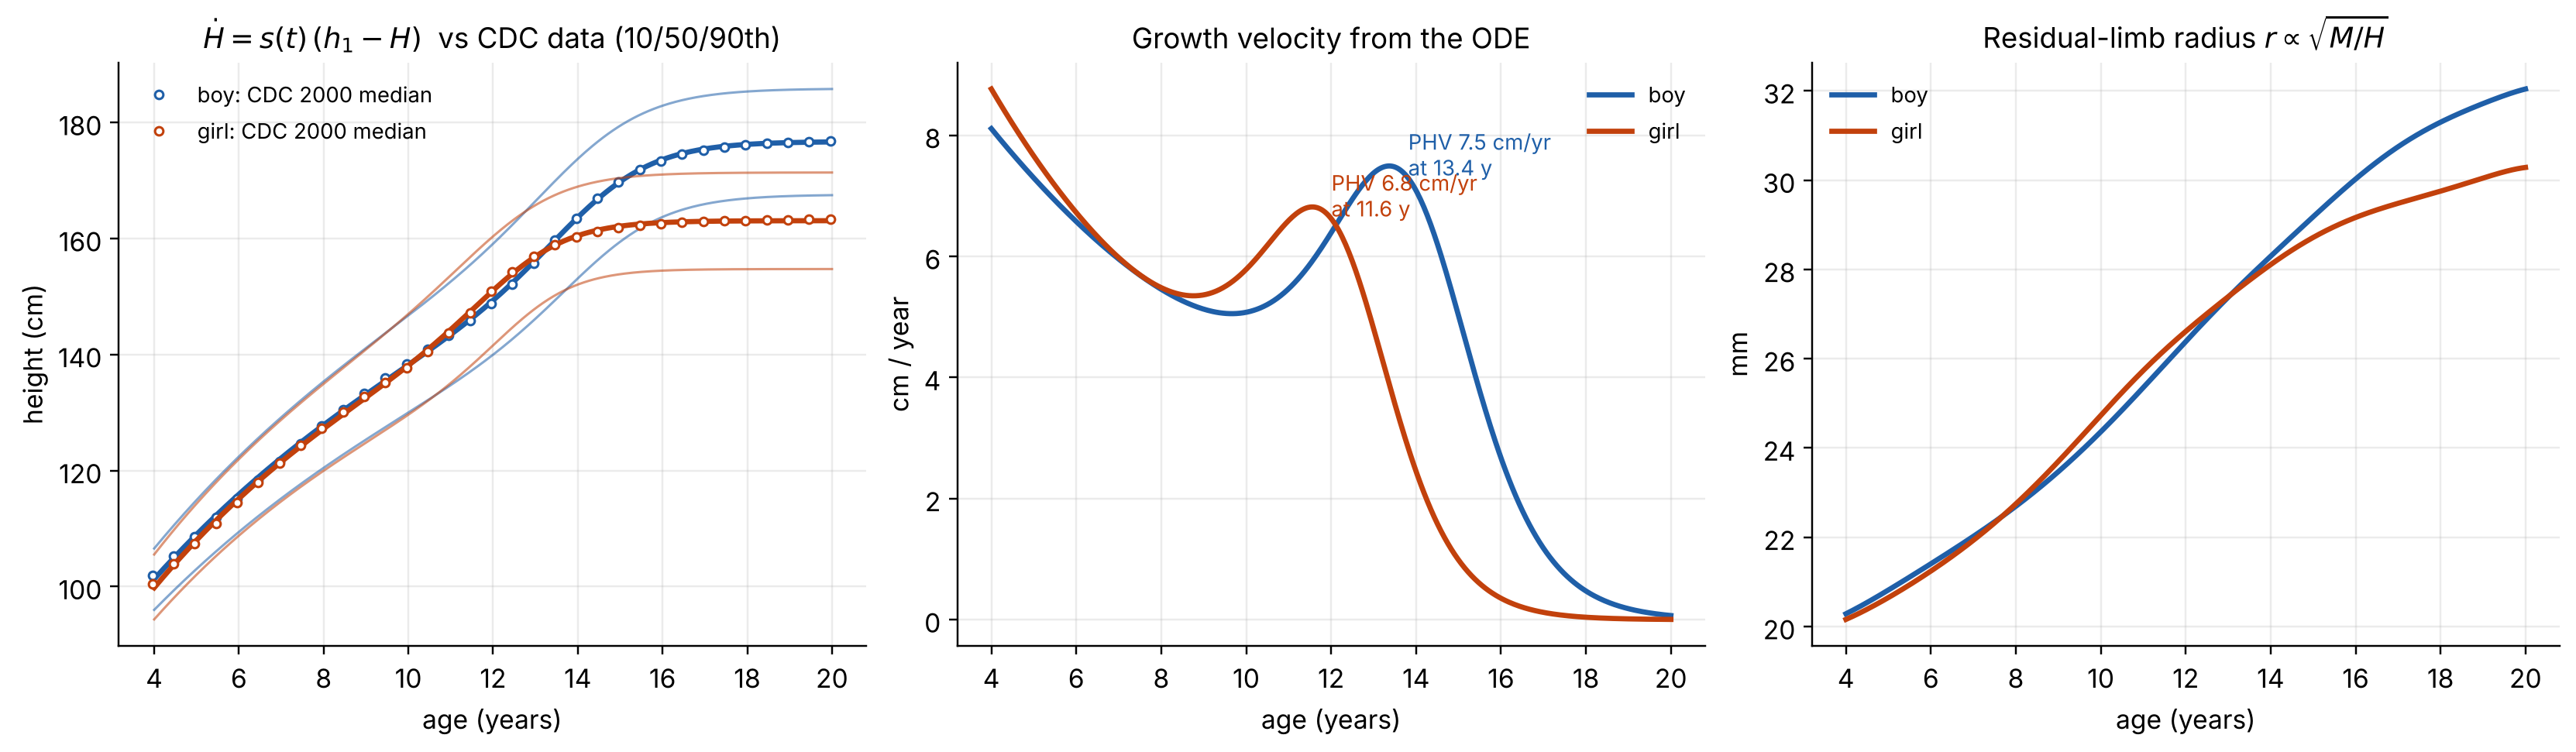
\includegraphics[width=\textwidth]{fig01_growth}
\caption{Growth layer. Left: ODE solution against CDC data (bold: median; thin: 10th/90th centiles). Centre: growth velocity. Right: residual-limb radius.}
\label{fig:growth}
\end{figure}

\section{Model 0: static mechanics of the socket}\label{sec:static}
Consider the simplest action: holding an object with the elbow at $90^\circ$. The distal body $D$ (prosthesis of mass $m_p$ with centre of mass at $x_p$, plus object $m_o$ at the grip distance $L_p$) is held by the residual limb, which is engaged in the socket over a length $L$ (Fig.~\ref{fig:fbd}). The limb must supply a shear force $V$ and a moment $M_B$ about the socket brim:
\begin{equation}
V=g\,(m_p+m_o),\qquad M_B=g\,(m_p x_p+m_o L_p).
\end{equation}
We assume the transverse line load $q(z)$ along the engaged length is linear, $q=q_0+q_1z$. Force and moment balance, $\int_0^Lq\,dz=V$ and $\int_0^Lzq\,dz=M_B$, give the edge loads
\begin{equation}
q(0)=\frac{4V}{L}-\frac{6M_B}{L^2},\qquad q(L)=-\frac{2V}{L}+\frac{6M_B}{L^2}.
\label{eq:edges}
\end{equation}
If the pressure is distributed as $p_0\cos\vartheta$ over the loaded half-circumference, then $q=\tfrac{\pi}{2}rp_0$, so the peak pressure is
\begin{equation}
p_{\mathrm{mom}}=\frac{2\max\{|q(0)|,|q(L)|\}}{\pi r}\;\approx\;\frac{12\,M_B}{\pi r L^2}.
\label{eq:pmom}
\end{equation}
The leading-order form shows the key sensitivity: pressure scales with the inverse \emph{square} of the engaged length, which is why short residual limbs are fragile. For a boy fitted at~8, \eqref{eq:edges}--\eqref{eq:pmom} give \staticEight\,kPa; the leading-order form is within \leadingError\% of the exact value over ages 5--17.

\begin{figure}[t]\centering
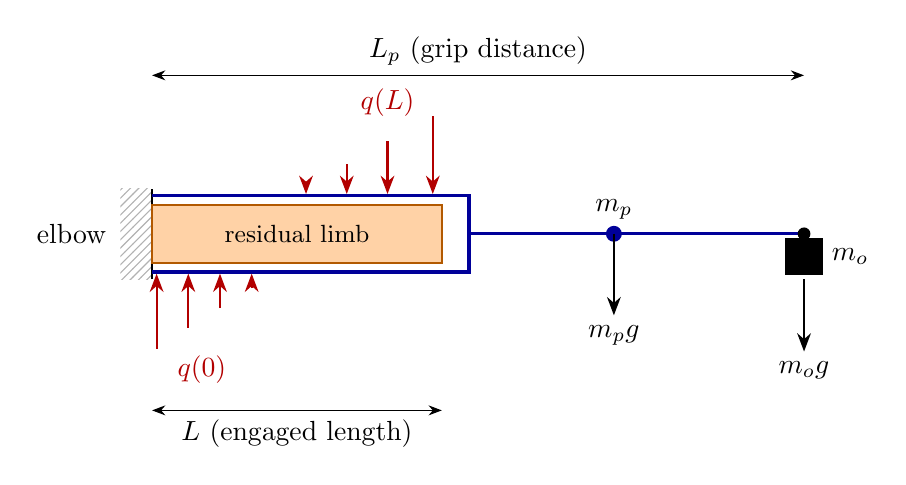
\begin{tikzpicture}[scale=1.15,>=Stealth]
\fill[pattern=north east lines,pattern color=gray!60] (-0.35,-0.5) rectangle (0,0.5);
\draw[thick] (0,-0.5)--(0,0.5);
\node[left] at (-0.4,0) {elbow};
\fill[orange!35] (0,-0.32) rectangle (3.2,0.32);
\draw[orange!70!black,thick] (0,-0.32) rectangle (3.2,0.32);
\node at (1.6,0) {\small residual limb};
\draw[very thick,blue!60!black] (0,0.42)--(3.5,0.42)--(3.5,-0.42)--(0,-0.42);
\draw[very thick,blue!60!black] (3.5,0)--(7.2,0);
\fill (7.2,0) circle (2pt);
\draw[fill=black] (7.0,-0.45) rectangle (7.4,-0.05);
\node[right] at (7.4,-0.25) {$m_o$};
\fill[blue!60!black] (5.1,0) circle (2.5pt);
\node[above] at (5.1,0.05) {$m_p$};
\draw[->,thick] (5.1,0)--(5.1,-0.9) node[below] {$m_pg$};
\draw[->,thick] (7.2,-0.5)--(7.2,-1.3) node[below] {$m_og$};
\foreach \x/\h in {0.05/0.85,0.4/0.62,0.75/0.4,1.1/0.18} {\draw[->,red!70!black,thick] (\x,-0.42-\h)--(\x,-0.44);}
\foreach \x/\h in {1.7/0.1,2.15/0.35,2.6/0.6,3.1/0.88} {\draw[->,red!70!black,thick] (\x,0.42+\h)--(\x,0.44);}
\node[red!70!black] at (0.55,-1.5) {$q(0)$};
\node[red!70!black] at (2.6,1.45) {$q(L)$};
\draw[<->] (0,-1.95)--(3.2,-1.95) node[midway,below] {$L$ (engaged length)};
\draw[<->] (0,1.75)--(7.2,1.75) node[midway,above] {$L_p$ (grip distance)};
\end{tikzpicture}
\caption{Free-body diagram of Model~0. The weights of the prosthesis and object create a shear force and a moment that the socket must transfer to the limb as a linearly varying line load (red): the socket presses up on the underside of the limb near the brim and down on its top surface near the distal end. With the forearm horizontal and the palm up, these are the posterior-proximal and anterior-distal regions.}
\label{fig:fbd}
\end{figure}

\paragraph{Scaling laws.} For a socket fitted at a given age, $L_p/L$ is a constant, $L\propto H$ and $r\propto\sqrt{M/H}$, so $rL\propto\sqrt{MH}$. Equations \eqref{eq:edges}--\eqref{eq:pmom} are linear in the masses, so
\begin{equation}
p_{\mathrm{mom}}=\underbrace{\frac{a\,m_p}{\sqrt{MH}}}_{\text{prosthesis}}+\underbrace{\frac{b\,m_o}{\sqrt{MH}}}_{\text{object}},
\end{equation}
with constants $a,b$. For a fixed object ($m_o$ constant) the whole pressure falls as $(MH)^{-1/2}$: a growing child copes better with the same bottle. If the object grows with the child ($m_o=fM$), the object term rises as $(M/H)^{1/2}$. Our numerical exponents are \slopeFixed\ and \slopeObject\ (Fig.~\ref{fig:static}), confirming the derivation exactly. The competition between the two terms is the seed of the window closure found in \S\ref{sec:policy}.

\begin{figure}[t]\centering
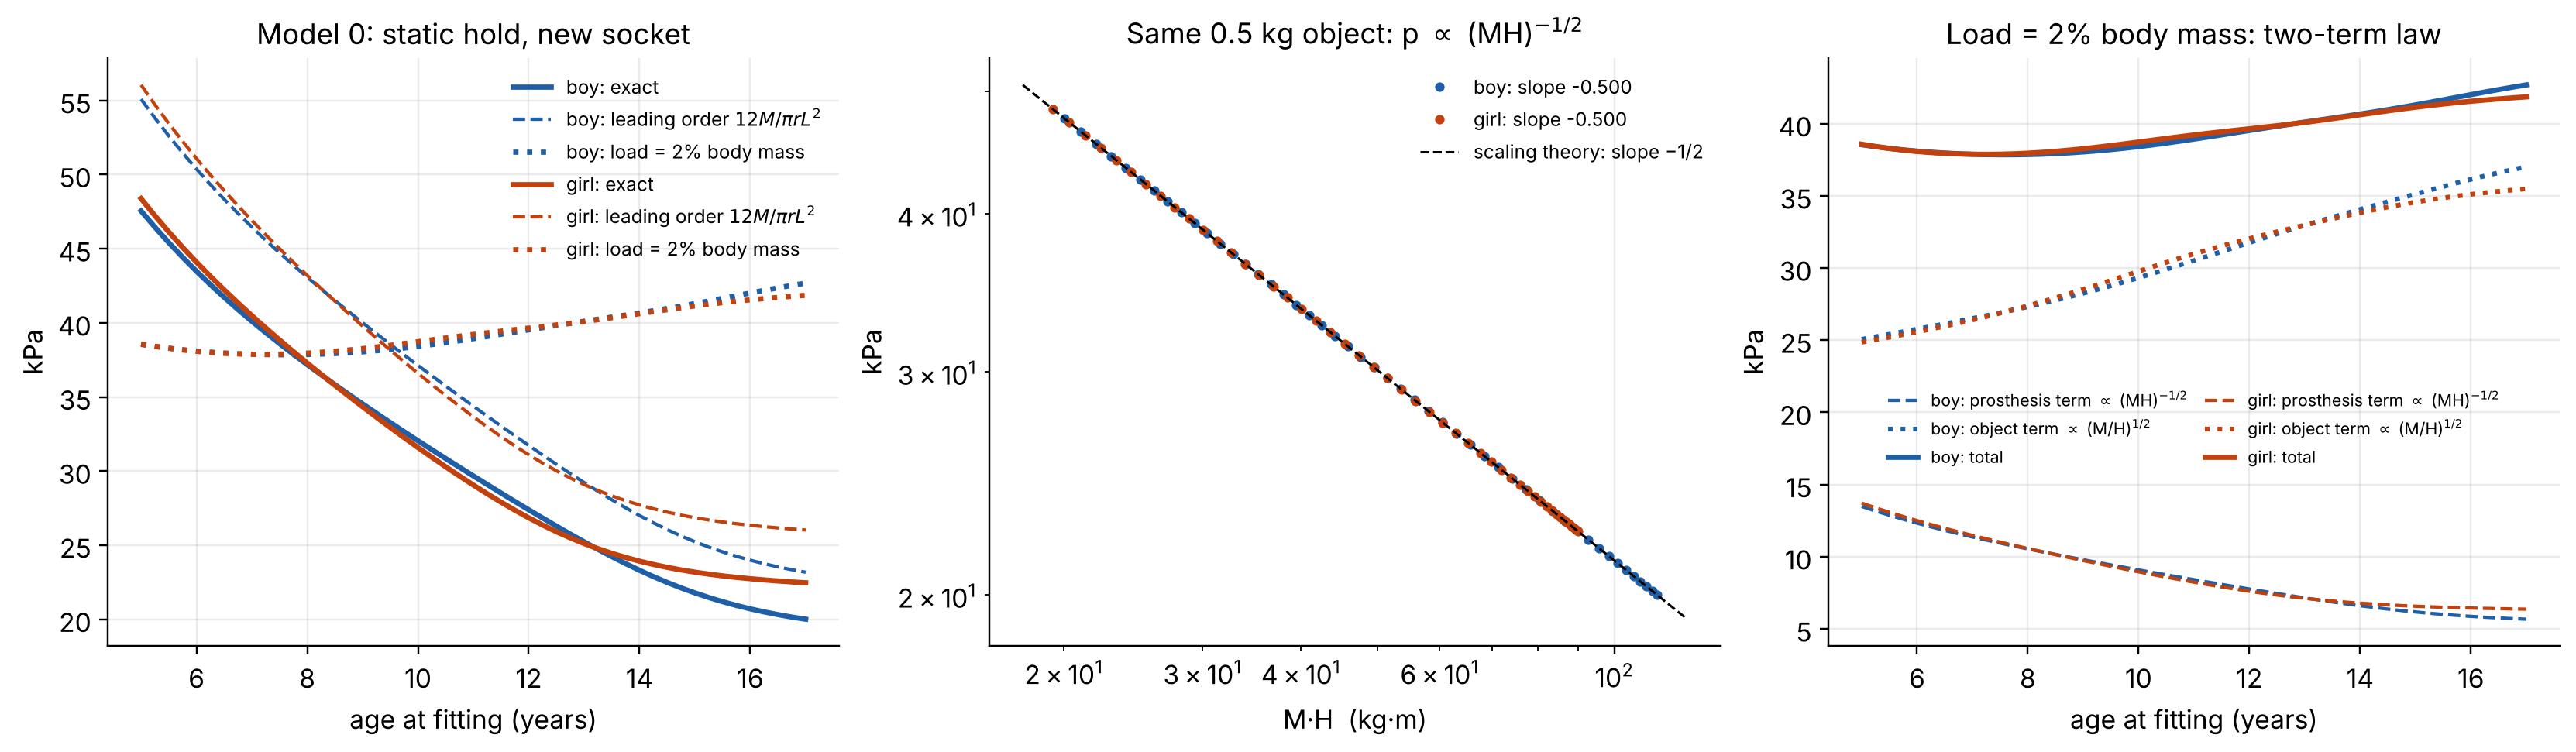
\includegraphics[width=\textwidth]{fig02_static_model}
\caption{Model~0 for a new socket at each age. Left: exact vs.\ leading-order pressure. Centre: fixed object, slope $-1/2$. Right: object scaled with body mass; the falling prosthesis term and rising object term.}
\label{fig:static}
\end{figure}

\section{Model 1: lifting dynamics}\label{sec:dynamics}
\paragraph{Action set.} We designed four simple actions (Fig.~\ref{fig:actions}): a static hold at $90^\circ$ elbow flexion; a slow curl ($10^\circ\!\to\!130^\circ$ elbow, 1.2\,s); the same curl performed fast (0.5\,s); and a lift to a shelf ($10^\circ\!\to\!100^\circ$ shoulder flexion, 1.2\,s). Each joint follows a minimum-jerk path \citep{flash1985}, $q(\tau)=q_0+\Delta q\,(10\tau^3-15\tau^4+6\tau^5)$, which is smooth, human-like and has peak angular acceleration $\tfrac{10}{\sqrt3}\,\Delta q/T^2$.

\begin{figure}[t]\centering
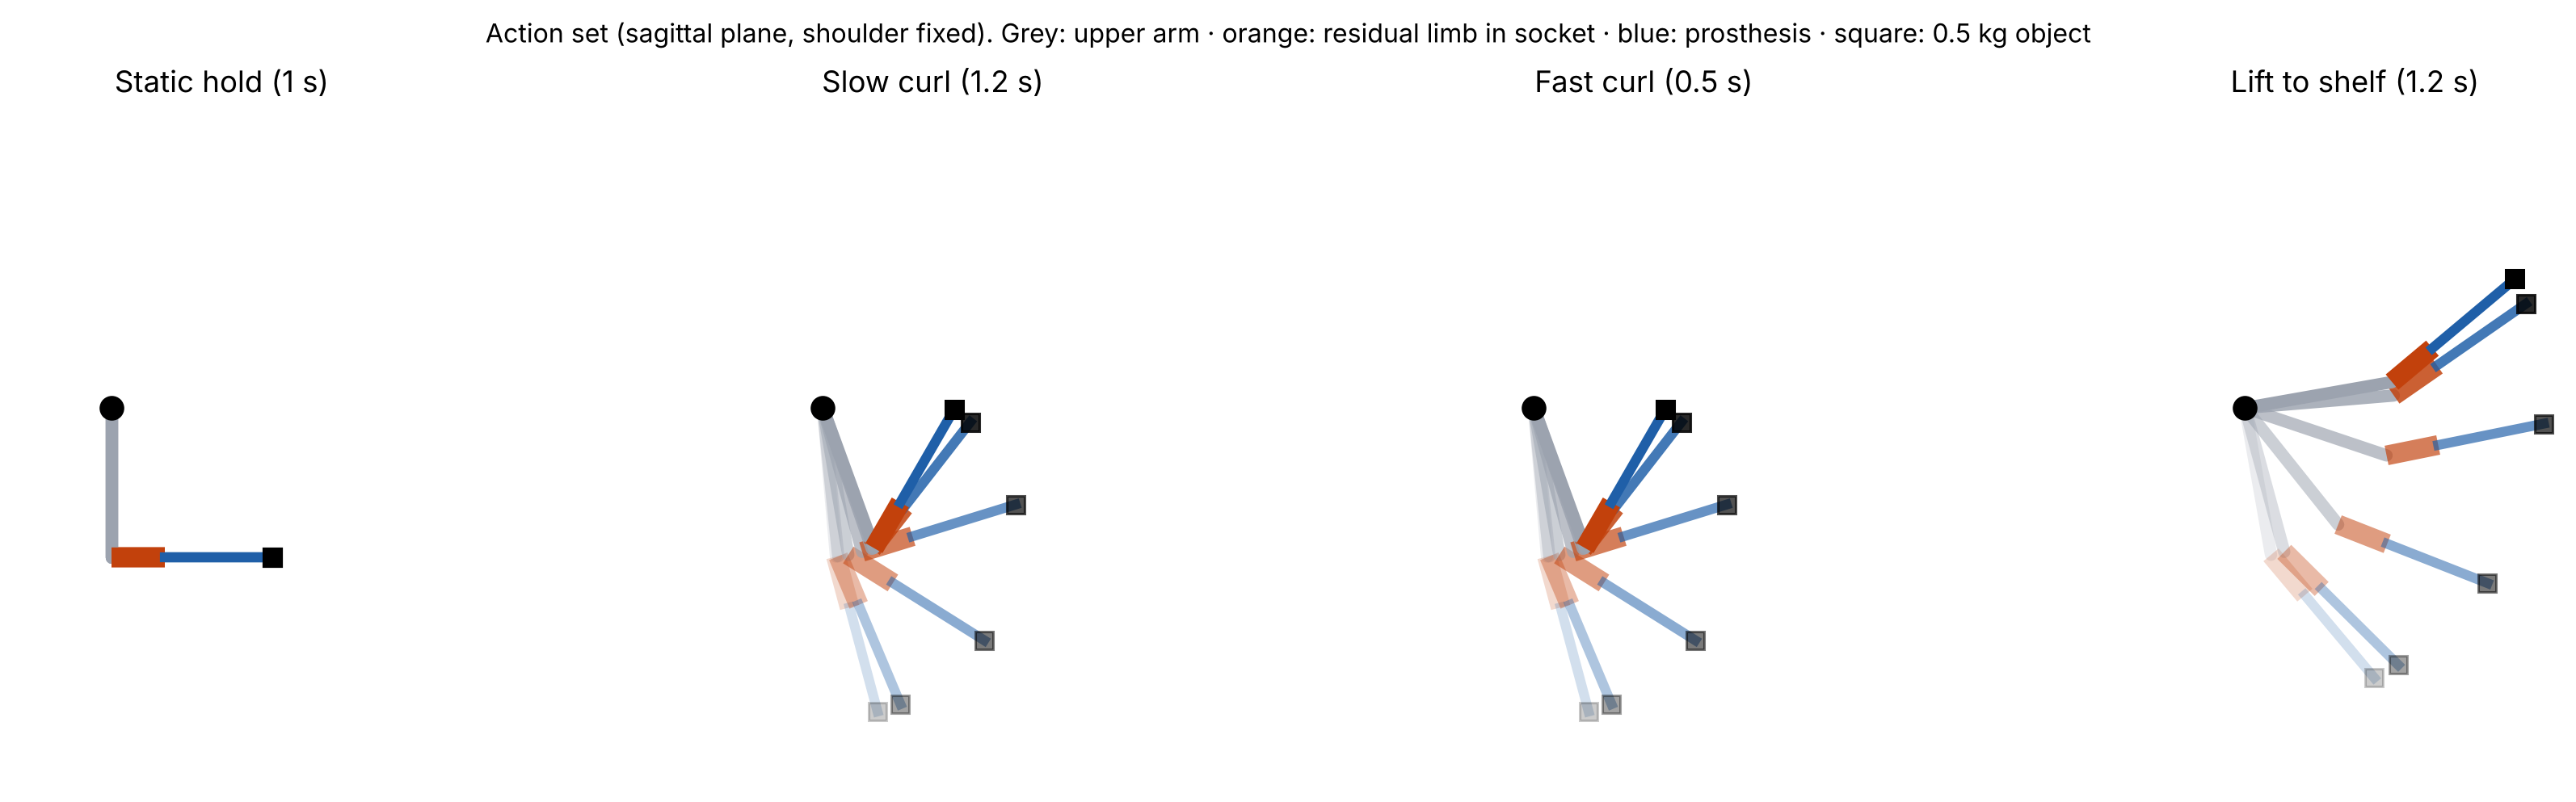
\includegraphics[width=\textwidth]{fig03_actions}
\caption{The four lifting actions for a boy fitted at age 8.}
\label{fig:actions}
\end{figure}

\paragraph{Equations of motion.} With shoulder angle $q_1$ measured from vertical and elbow flexion $q_2$, the Lagrangian of the two-link arm gives \citep{spong2006}
\begin{equation}
\mathbf{M}(q_2)\,\ddot{\mathbf q}+\mathbf C(\mathbf q,\dot{\mathbf q})+\mathbf G(\mathbf q)=\bm\tau,
\end{equation}
\begin{align*}
M_{11}&=I_1+m_1c_1^2+I_2+m_2(L_1^2+c_2^2+2L_1c_2\cos q_2), & M_{12}&=I_2+m_2(c_2^2+L_1c_2\cos q_2),\\
M_{22}&=I_2+m_2c_2^2, & h&=m_2L_1c_2\sin q_2,\\
C_1&=-h(2\dot q_1\dot q_2+\dot q_2^2), & C_2&=h\dot q_1^2,\\
G_1&=g[m_1c_1\sin q_1+m_2(L_1\sin q_1+c_2\sin(q_1+q_2))], & G_2&=g\,m_2c_2\sin(q_1+q_2).
\end{align*}
Link~2 lumps the residual limb, the prosthesis and the object. The socket loads come from Newton--Euler on the distal body $D$: $\mathbf F=\sum_i m_i(\mathbf a_i-\mathbf g)$ and $M_B=\sum_i(x_i-s)\,\hat{\mathbf u}\times m_i(\mathbf a_i-\mathbf g)+I_D\ddot\varphi$, projected onto the forearm axis (pull-out force $A$) and its normal (shear $V$), and then converted to pressure with \eqref{eq:edges}--\eqref{eq:pmom}.

\paragraph{Results.} At fitting, the static hold, slow curl, lift to shelf and fast curl produce peak pressures of \pHold, \pSlow, \pShelf\ and \pFast\,kPa (Fig.~\ref{fig:loads}). The fast curl nearly doubles the load of the static hold with the \emph{same} object, so speed, not weight, is the critical feature of the action set.

\paragraph{Dimensionless collapse.} The inertial moment relative to the gravitational one is measured by
\begin{equation}
\Pi=\frac{10}{\sqrt3}\,\frac{\Delta q\,L_p}{g\,T^2}.
\end{equation}
We simulated both curls for 8 children (both sexes, ages 6--15) at 6 speeds, \piAllN\ runs in all. The ratio of peak dynamic to static pressure follows $\collapseA+\collapseB\,\Pi$ closely ($R^2=\collapseR$, Fig.~\ref{fig:collapse}). The slope is close to 1, which is what we would expect from a number that compares inertial and gravitational load. The intercept needs care, because it belongs to the straight line and not to the physics. For slow curls ($\Pi<\piLowCut$, \piLowN\ of the \piAllN\ runs) the ratio is \piLowMin--\piLowMax: a slow curl loads the socket just like holding the object still, because the peak comes when the forearm passes through the horizontal. So the real curve is flat near 1 for small $\Pi$ and then rises roughly in step with $\Pi$. One line fits the whole cloud well because most of the range is at large $\Pi$, but it misses the flat start by up to \piLineErr. In practice: \emph{below $\Pi\approx0.3$ the speed of the movement hardly matters; above it, socket load grows roughly linearly with $\Delta q/T^2$.}

\begin{figure}[t]\centering
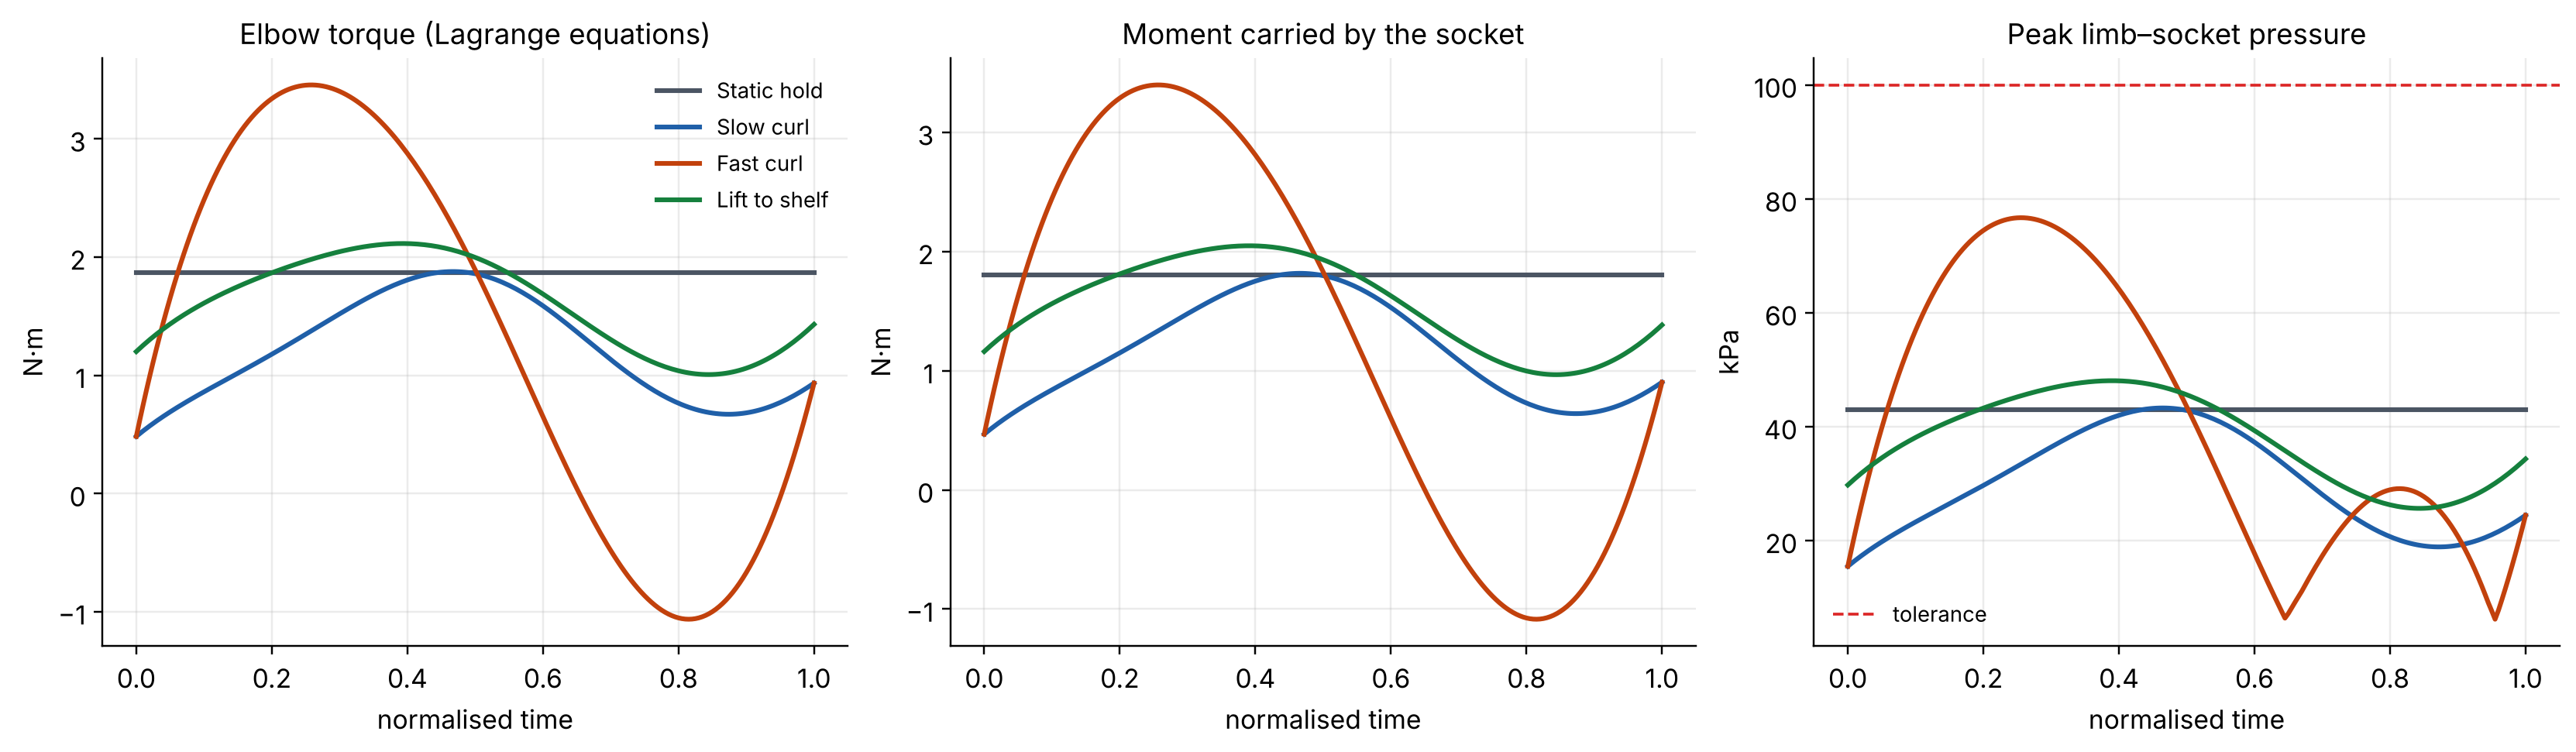
\includegraphics[width=\textwidth]{fig04_task_loads}
\caption{Elbow torque, socket moment and peak pressure during each action (boy fitted at 8).}
\label{fig:loads}
\end{figure}
\begin{figure}[t]\centering
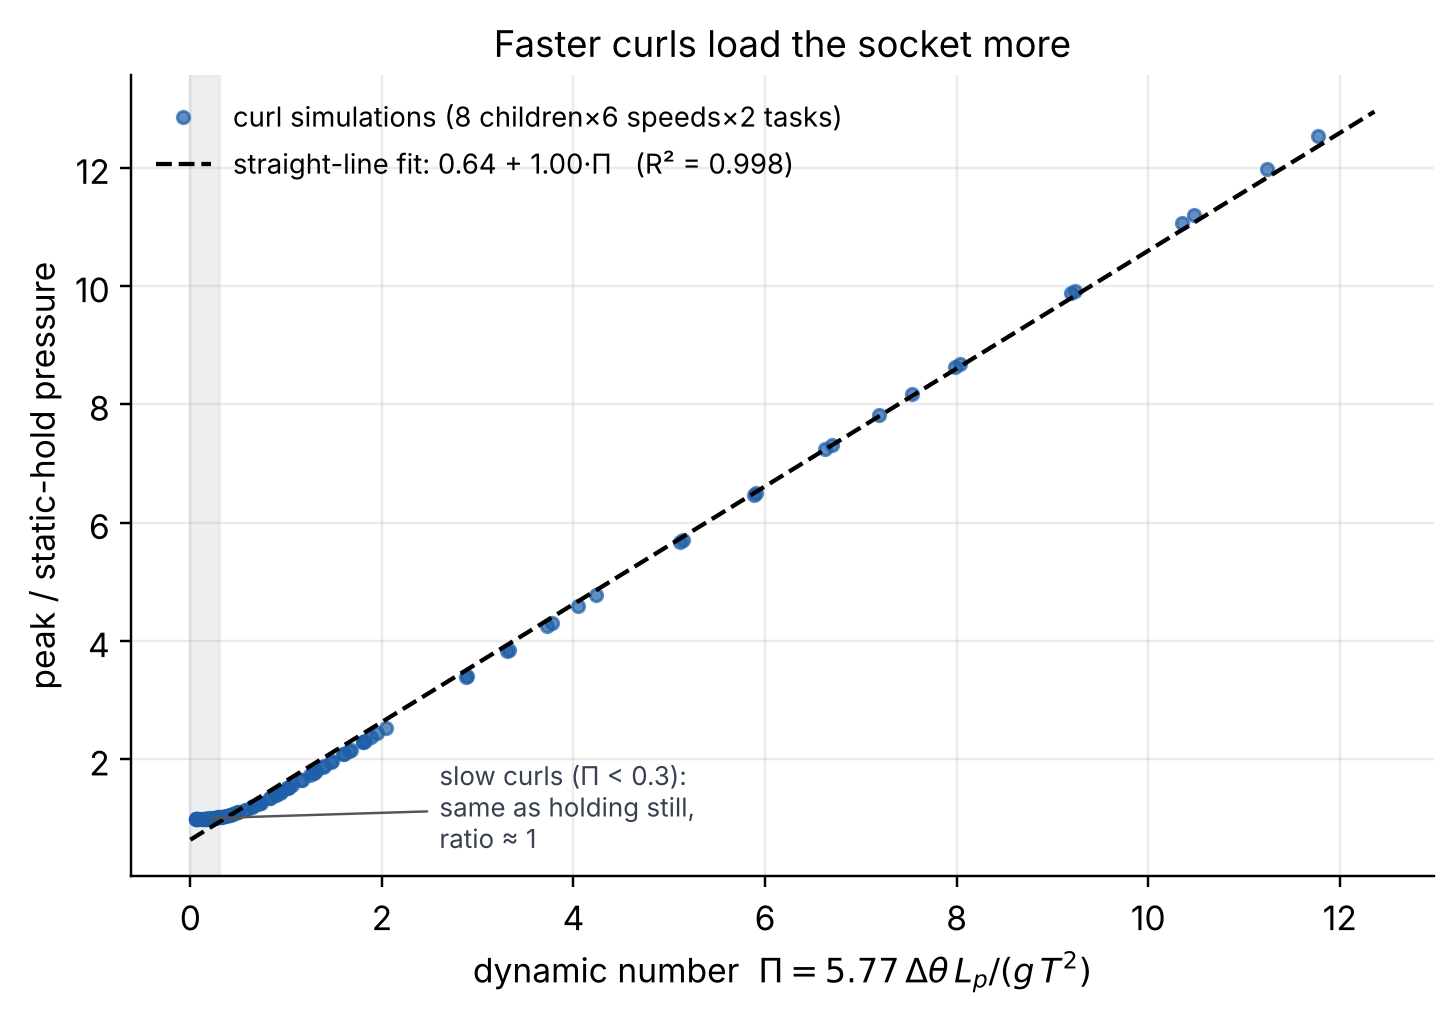
\includegraphics[width=0.55\textwidth]{fig05_dynamic_collapse}
\caption{Dynamic amplification against the dimensionless number $\Pi$. The dashed line is a straight-line fit to all runs. Slow curls (grey band) sit at a ratio of 1, so the line should not be read down to $\Pi=0$.}
\label{fig:collapse}
\end{figure}

\section{Model 2: coupling the interface to growth}\label{sec:coupling}
After fitting at age $t_f$ the socket is frozen while the limb changes:
\begin{equation}
\ell_r(t)=\ell_r(t_f)+\phi\,[\ell_f(t)-\ell_f(t_f)],\qquad
\varepsilon(t)=\frac{r(t)-r_s}{0.4\,r(t)},\qquad
p_{\mathrm{fit}}=\frac{E}{B}\left(e^{B\varepsilon}-1\right).
\end{equation}
If the residual limb outgrows the socket depth, it bottoms out and pushes the socket distally by $s=\max(0,\ell_r-d)$, which lengthens the lever arm. Peak pressure is $p_{\mathrm{peak}}=p_{\mathrm{fit}}+p_{\mathrm{mom}}$, and we define the Socket Stress Index $\Ssi=p_{\mathrm{peak}}/p_{\mathrm{tol}}$.

\paragraph{Two competing interface mechanisms.}
\emph{Cylindrical socket:} growth only compresses the tissue. \emph{Tapered socket} (half-angle $\alpha=4^\circ$): once the interference pressure exceeds what the child can push against when donning,
\begin{equation}
p_{\mathrm{don}}=\frac{F_{\mathrm{don}}}{2\pi rL\,(\mu\cos\alpha+\sin\alpha)},
\end{equation}
the limb sits proud of the socket by a ride-up $s$. This relieves interference by $s\tan\alpha$ but shortens the engaged length to $L=\ell_r-s$. We solve $p_{\mathrm{fit}}(s)=p_{\mathrm{don}}(L(s))$ for $s$ with Brent's method.

\paragraph{Results.} For a boy fitted at~8 the two mechanisms fail in opposite ways (Fig.~\ref{fig:single}). In the cylindrical socket, lifting causes \liftShare\% of the pressure on day one, but tissue compression rises exponentially and reaches \fitShareFail\% of the peak at failure after \lifeCyl\ months. In the tapered socket, fit pressure stays capped, but the limb rides up \rideUpFail\,mm, the engaged length falls from \engagedMM\ to \engagedFail\,mm, and by \eqref{eq:pmom} the lifting pressure takes over after \lifeTap\ months. Across fitting ages 5--12 the model gives lifetimes between 13.5 and 37 months, depending on sex, socket type and age at fitting (Fig.~\ref{fig:lifemap}), and the tapered socket always fails first. Section~\ref{sec:validation} compares these lifetimes with clinical replacement records.

\begin{figure}[t]\centering
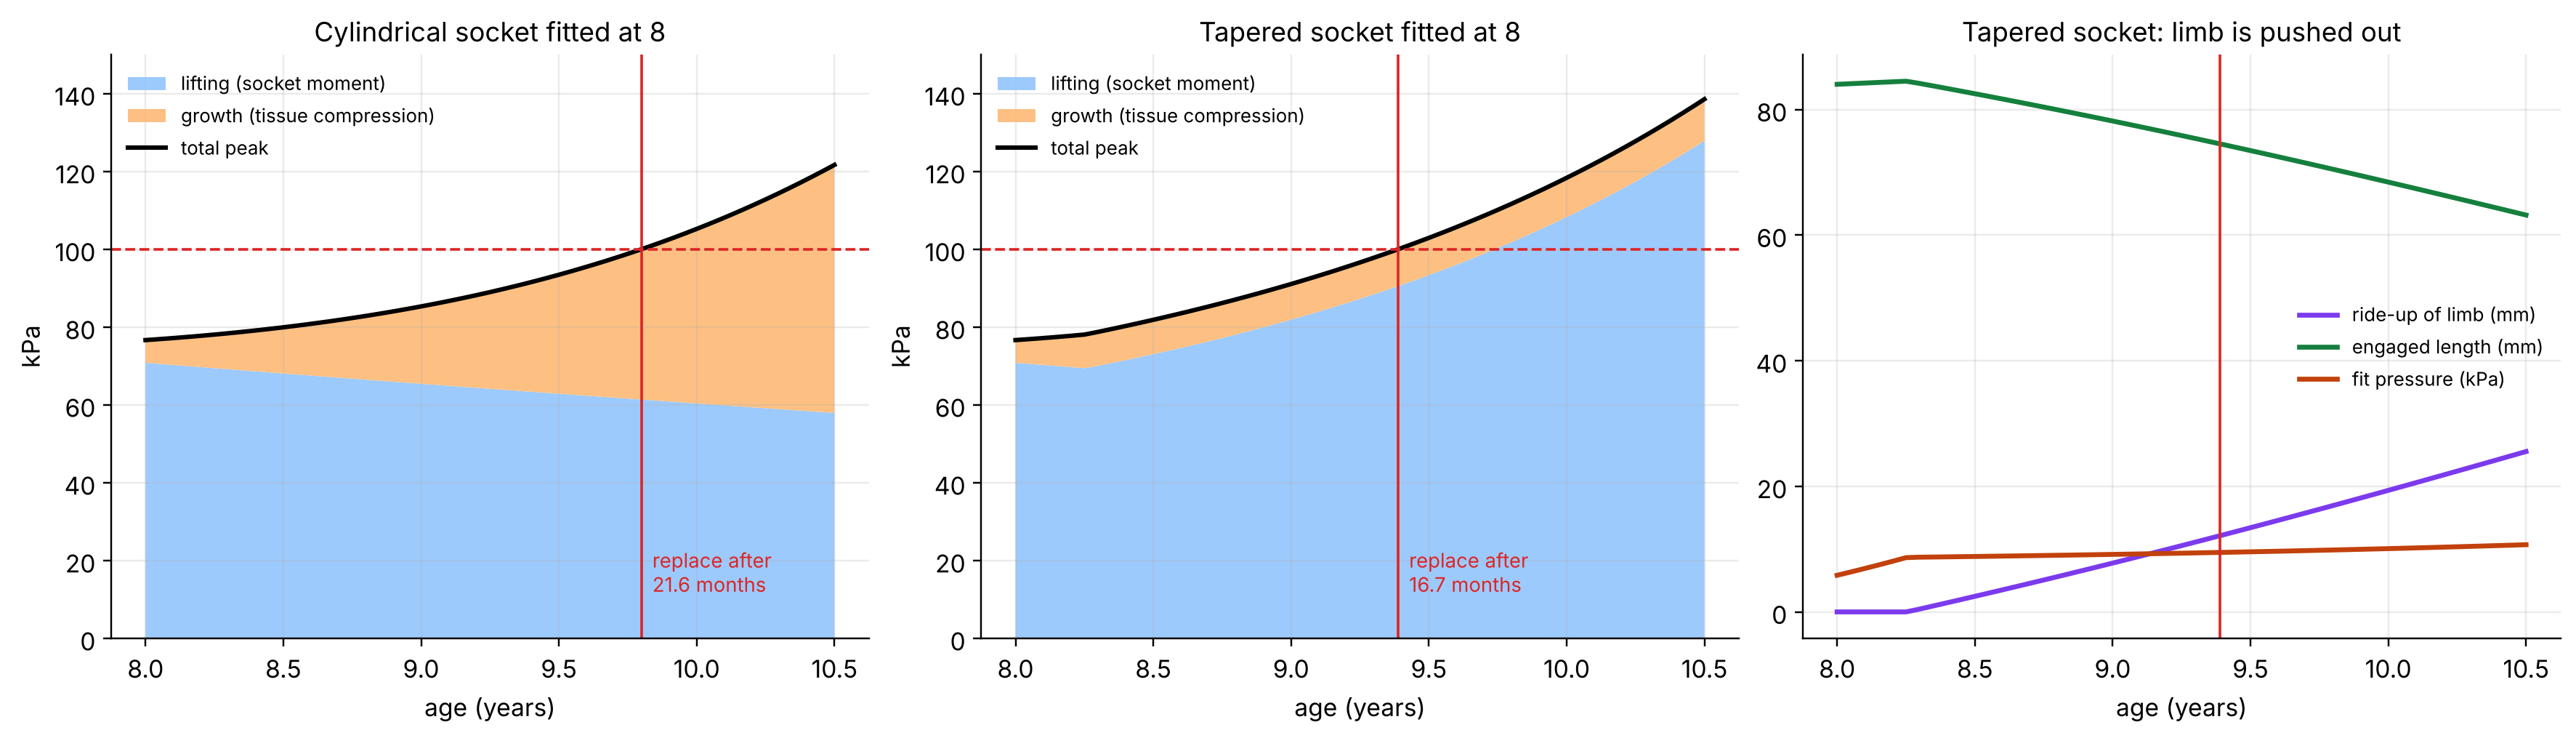
\includegraphics[width=\textwidth]{fig06_single_socket}
\caption{A single socket fitted at age 8. Cylindrical (left) and tapered (centre) sockets reach the tolerance through different mechanisms. Right: the tapered socket is pushed off the limb.}
\label{fig:single}
\end{figure}
\begin{figure}[t]\centering
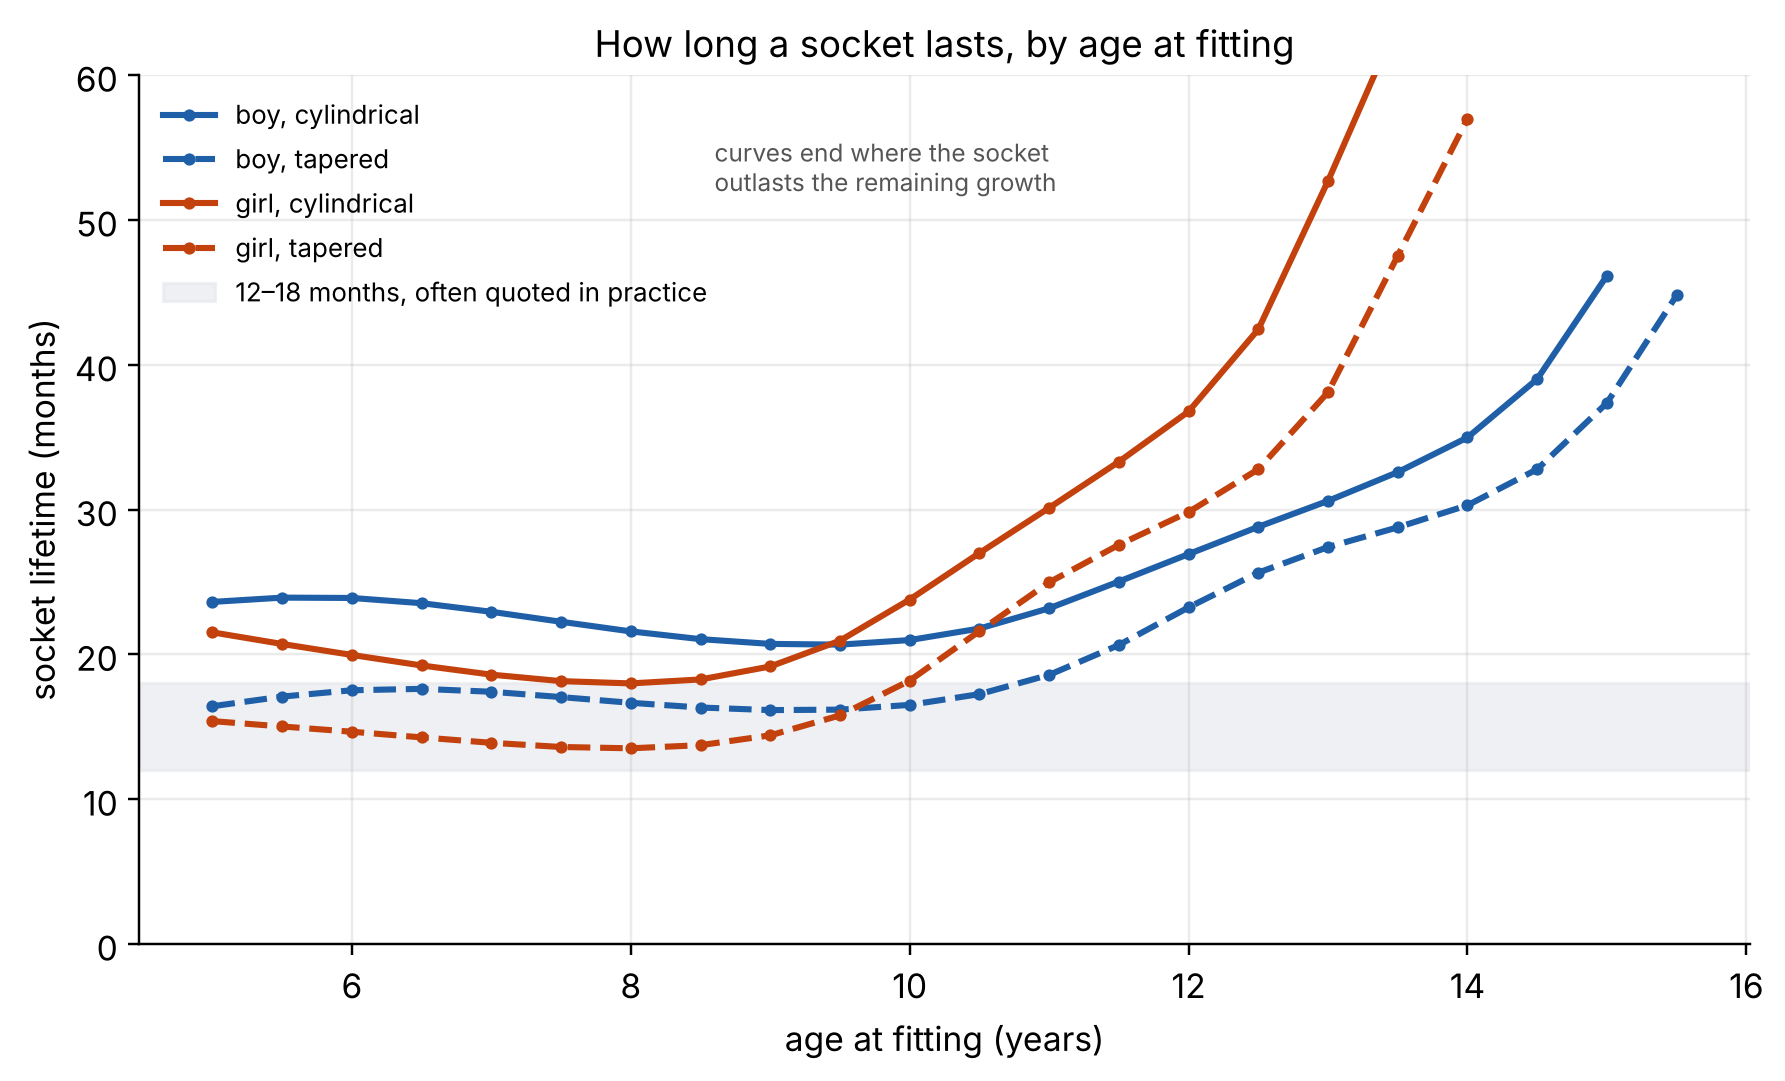
\includegraphics[width=0.62\textwidth]{fig07_lifetime_map}
\caption{Socket lifetime against age at fitting.}
\label{fig:lifemap}
\end{figure}

\section{The slow system as ODEs, with failure as an event}\label{sec:ode}
\paragraph{Two time scales.} An action lasts 0.5--1.2\,s and a socket lasts about two years. The ratio of the fast to the slow time is $\timeRatio$ for the fast curl, so during one action the limb is frozen, and over the life of the socket the arm dynamics matter only through their peak response. The arm is the fast subsystem (Section~\ref{sec:dynamics}). We eliminate it adiabatically and keep its peak lifting pressure $p_{\mathrm{lift}}(t)$, evaluated from the Lagrange model at the current body size, as a slowly varying forcing.

\paragraph{Slow system.} For a cylindrical socket fitted at $t_f$ with fit strain $\varepsilon_0$, so that its radius is fixed at $r_s=r(t_f)(1-\beta\varepsilon_0)$ with $\beta=0.4$ the soft-tissue fraction, the state $(H,\ell_r,r,\varepsilon,p_{\mathrm{fit}})$ obeys
\begin{align}
\dot H &= s(t)\,(h_1-H), &
\dot\ell_r &= \phi f_f\,\dot H, \label{eq:ode1}\\
\dot r &= \tfrac12\,r\left(\frac{\dot M}{M}-\frac{\dot H}{H}\right), &
\dot\varepsilon &= \left(\frac1\beta-\varepsilon\right)\frac{\dot r}{r}, \label{eq:ode2}\\
\dot p_{\mathrm{fit}} &= (E+B\,p_{\mathrm{fit}})\,\dot\varepsilon, \label{eq:ode3}
\end{align}
where $M(t)$ is the CDC weight centile and $f_f=0.146$ the forearm-to-height ratio. The equation for $\dot\varepsilon$ follows from $\varepsilon=(r-r_s)/(\beta r)$ with $r_s$ constant; the last equation follows from differentiating the tissue law, $dp/d\varepsilon=E+Bp$. The socket is replaced at the first event
\begin{equation}
p_{\mathrm{fit}}(t)+p_{\mathrm{lift}}(t)=p_{\mathrm{tol}}\ \ \text{(pressure)},\qquad
\mu\,p_{\mathrm{fit}}\,A_c(t)=F_{\mathrm{pull}}(t)\ \ \text{(suspension)},
\end{equation}
where $A_c=2\pi r(\ell_r-s)$ is the contact area and $F_{\mathrm{pull}}$ the pull-out force of the worst action. We integrate with an adaptive Dormand--Prince method (relative tolerance $10^{-9}$) and locate each event by root-finding on the dense output. Suspension never ended a socket's life during growth in the cases we ran; it fires only on the day of fitting for fits that are too loose. The tapered socket adds an algebraic seating constraint (Section~\ref{sec:coupling}), which makes it a differential--algebraic problem, and for it we keep the scan-and-bisect search.

\paragraph{A conserved quantity and a girth budget.} Equations \eqref{eq:ode2} give $\tfrac{d}{dt}\big[(1-\beta\varepsilon)\,r\big]=0$, so the squeeze is fixed by cumulative girth growth alone: $r(t)/r_0=(1-\beta\varepsilon_0)/(1-\beta\varepsilon(t))$. A socket therefore has a \emph{girth budget}. If $\varepsilon^*=\tfrac1B\ln\!\big(1+B\,(p_{\mathrm{tol}}-p_{\mathrm{lift}})/E\big)$ is the strain at which tissue pressure fills the headroom left by lifting, the socket survives until
\begin{equation}
\frac{r}{r_0}=R^*=\frac{1-\beta\varepsilon_0}{1-\beta\varepsilon^*}.
\label{eq:budget}
\end{equation}
For a boy fitted at 8 with a 5\% fit, $R^*-1$ is \budgetLo\% if we use the lifting pressure of day one and \budgetHi\% if we use its end-of-life value (the fixed 0.5\,kg object becomes relatively lighter as the child grows). Girth grows by \girthRate\% per year over this socket's life, so the lifetime is $\ln R^*/\langle d\ln r/dt\rangle$, between \bracketLo\ and \bracketHi\ months; the larger value is the event time (\eventMonths\ months, Fig.~\ref{fig:ode}). A socket made for a 5\% squeeze is therefore finished by only 5--7\% of girth growth, and it is girth, not length, that ends its life.

\paragraph{Verification.} Along a whole socket life the ODE state agrees with the algebraic interface model of Section~\ref{sec:coupling} to a relative $\odeStateErr$ (height, length, radius, strain and fit pressure), and $(1-\beta\varepsilon)r$ drifts by only $\odeConserved$. The event time equals the scan-and-bisect lifetime to within \odeGap\ months in all \odeN\ cases we tried (both sexes, fitting ages 5--12, standard and patient-specific fits, and \odeSusp\ day-one suspension failures), with the same failure mode in each.

\begin{figure}[t]\centering
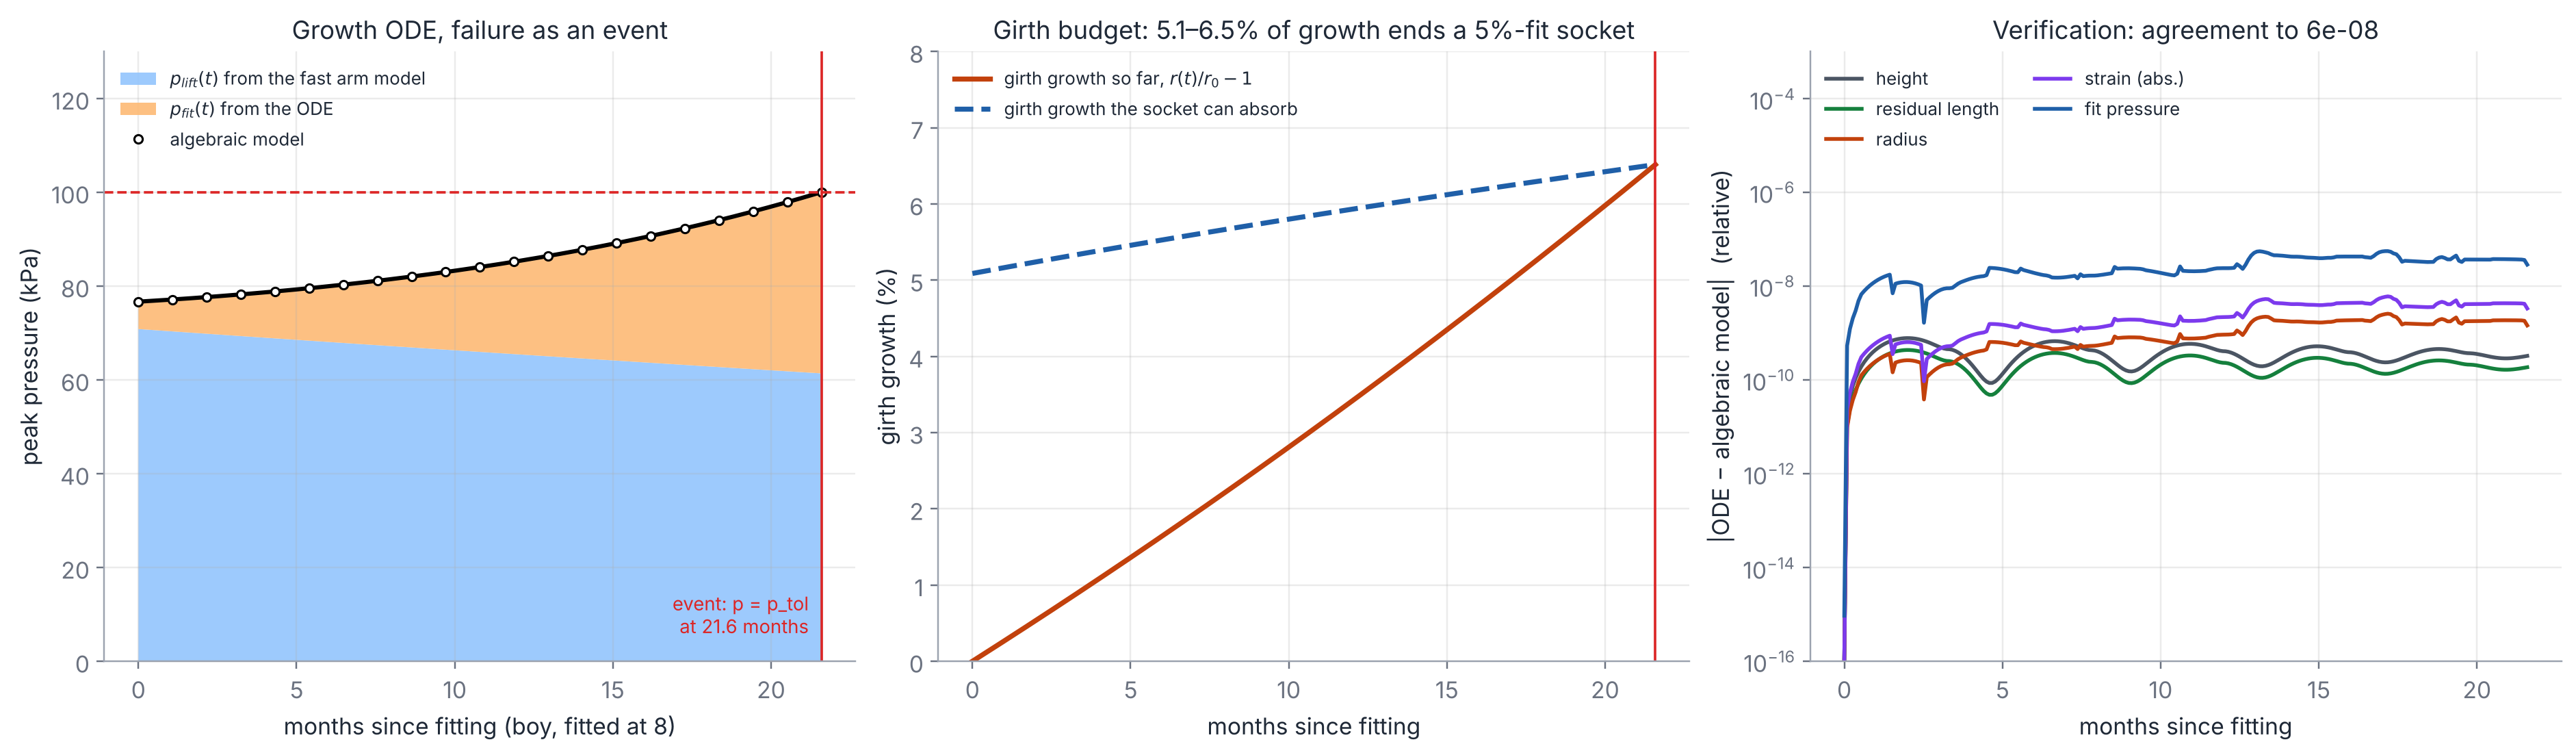
\includegraphics[width=\textwidth]{fig18_ode_formulation}
\caption{The slow system as an initial-value problem (boy fitted at 8). Left: ODE solution with the algebraic model overlaid (circles); the event is where total pressure reaches the tolerance. Centre: girth growth so far against the growth the socket can absorb, Eq.~\eqref{eq:budget}; the curves meet at the event. Right: the ODE and algebraic models agree to about $10^{-8}$.}
\label{fig:ode}
\end{figure}

\section{The point of substantial change}\label{sec:policy}
\paragraph{Routine replacement: the headroom law.} The pressure tolerance of a child's residual limb has not been measured, and the lifetimes above move a great deal with it (Fig.~\ref{fig:headroom}, centre: for a boy fitted at 8, tolerances of 80, 90, 100 and 120\,kPa give 6.1, 15.7, 21.6 and 29.5 months). The peak-pressure path $P(t)$ of a frozen socket, however, does not depend on the tolerance at all. A socket fails when $P$ reaches $p_{\mathrm{tol}}$, so its lifetime is $T(x)$, the time at which $P$ has risen by the fraction $x=p_{\mathrm{tol}}/P(0)-1$, the \emph{pressure headroom}. We therefore report the path. For a boy fitted at 8 with a standard fit, $P(0)=\pZeroEight$\,kPa, and in a cylindrical socket the peak pressure is 10, 25 and 50\% higher after \tTenBoyCyl, \tPlusBoyCyl\ and \tFiftyBoyCyl\ months. The $+25\%$ point comes after \tPlusBoyTap\ months in a tapered socket, \tPlusGirlCyl\ and \tPlusGirlTap\ months for a girl, and across fitting ages 6--12, both sexes and both socket types it lies between \tPlusMin\ and \tPlusMax\ months. Our assumed 100\,kPa is a headroom of \headroomBase\%, which is what gives \lifeCyl\ and \lifeTap\ months. Reading lifetimes off the path reproduces the original search to within \headroomGap\ months. This also suggests a protocol that needs no assumed tolerance: measure $P(0)$ at fitting, compare it with the clinician's own limit for that child, and use the path to book the next review.

\begin{figure}[t]\centering
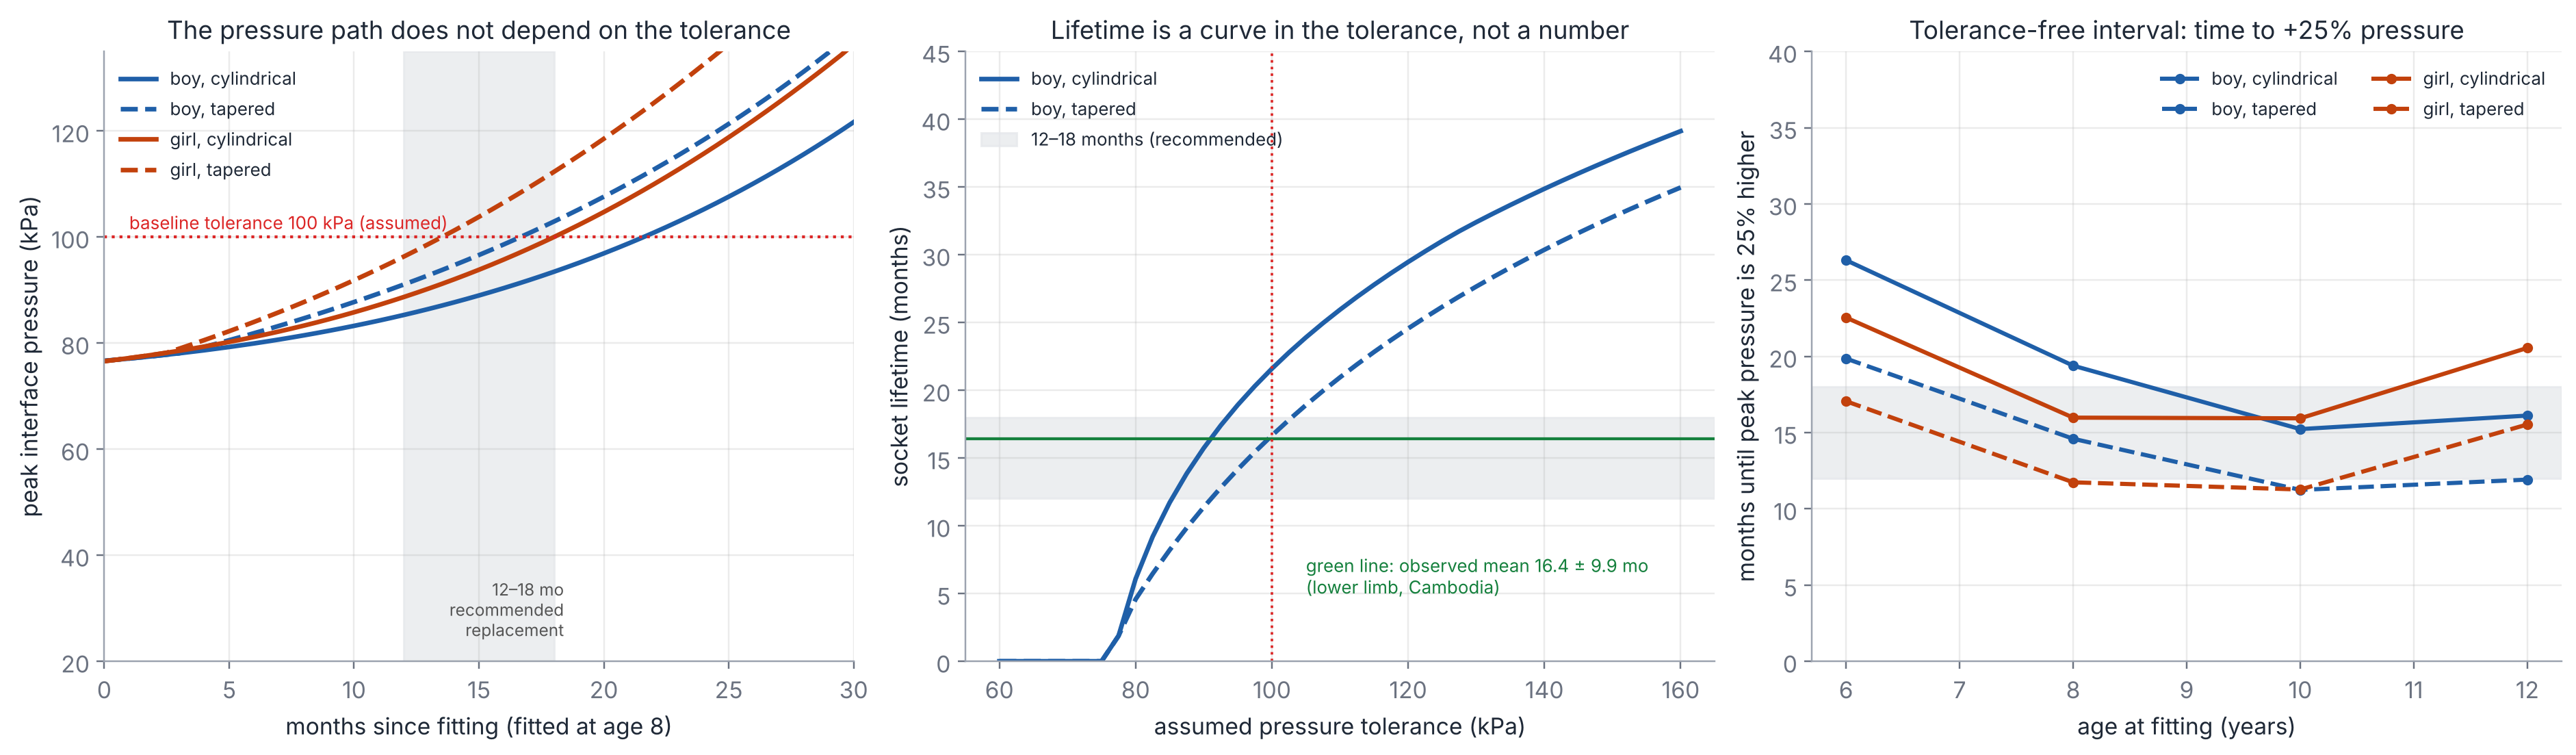
\includegraphics[width=\textwidth]{fig16_headroom_law}
\caption{Tolerance-free lifetime. Left: the peak-pressure path of a socket fitted at 8 for both sexes and socket types; the tolerance only decides where it is cut. Centre: lifetime as a function of the assumed tolerance, with the observed mean replacement interval of Ghidini et al.\ (green) and the recommended 12--18 months (grey). Right: months until the peak pressure is 25\% above its day-one value, by age at fitting.}
\label{fig:headroom}
\end{figure}

\paragraph{A cheaper policy.} Simulating every socket from age 6 to 18 (Fig.~\ref{fig:schedule}), a standard 5\% tissue-compression fit needs \socketsStdBoy\ sockets for a median boy. Fitting each socket instead at the loosest strain that still suspends the prosthesis with a safety factor of 1.25 (a growth allowance) needs \socketsGrowthBoy. That saves one fabrication and one clinic journey, which matters most in the remote settings described in the problem.

\paragraph{Window closure.} If the everyday load grows with the child (we use 2\% of body mass), then by \S\ref{sec:static} the object term rises as $(M/H)^{1/2}$. The pressure margin of a \emph{freshly fitted} socket therefore shrinks to zero at a finite age, the window-closure age. After it, refitting the same design cannot keep the child below tolerance during the action set (Fig.~\ref{fig:closure}). In our baseline, closure comes at \closureBoy\ years for median boys and \closureGirl\ years for median girls. For boys that is about half a year after peak height velocity (\phvAgeBoy\ y), but for girls it is about three years after it (\phvAgeGirl\ y), so it is not simply ``the growth spurt''. For 90th-centile children closure comes at \closureBoyNinety\ and \closureGirlNinety\ years, while 10th-centile boys reach it at \closureBoyTen\ years and 10th-centile girls not before 18. Only the fast curl sets this age: with that action removed there is no closure before 18 (Fig.~\ref{fig:firm}), so the result is really about brisk, loaded movements. What it calls for is a design change (longer socket trim lines, a different suspension, or a load-sharing harness), not just a larger socket. Because it depends on body size, screening should be triggered by size and residual-limb length, not by age alone.

\paragraph{How firm is that number?} Not very. We changed one assumption at a time and re-ran the closure search (Fig.~\ref{fig:firm}). If the object is 2.5\% of body mass instead of 2\%, closure moves to \sensLoadHighBoy\ years for boys and \sensLoadHighGirl\ for girls, and at 3\% to \sensLoadTopBoy\ and \sensLoadTopGirl. At 1.5\% there is no closure before 18. A pressure tolerance of 75\,kPa instead of 100 gives \sensTolLowBoy\ and \sensTolLowGirl\ years, while 125\,kPa again gives no closure. We also found an inconsistency in our own baseline. Every new socket is designed for a residual limb that is 45\% of the forearm at the age it is fitted, so the limb is assumed to be longer at 14 than the growth rule of Section~\ref{sec:coupling} would allow. If the limb follows that rule after age 8, closure comes at \sensLimbEightBoy\ and \sensLimbEightGirl\ years (\sensLimbSixBoy\ and \sensLimbSixGirl\ if the rule starts at 6). Letting the prosthesis mass grow with the child matters less: \sensMassBoy\ years for boys if it grows with height, \sensMassCubeBoy\ if it grows with height cubed. Two other assumptions matter more than any of these. The first is that the fast curl lasts 0.5\,s at every age. If a larger child moves proportionally slower, $T\propto H^{\kappa}$, closure moves later (Fig.~\ref{fig:hidden}): for boys from \kappaZeroBoy\ years at $\kappa=0$ to \kappaQuarterBoy\ at $\kappa=0.25$, and to no closure before 18 for $\kappa\ge0.35$ (for girls $\kappa\ge0.15$); $\kappa=0.5$ is dynamic similarity, in which $\Pi$ does not change with size. We know of no data that pin $\kappa$ down. The second is that the object share and the tolerance act, approximately, as one ratio, so a stiffer tolerance and a heavier everyday object offset each other (Fig.~\ref{fig:hidden}).

To combine all these uncertainties we drew \cloMcN\ Latin-hypercube samples of the nine inputs of Section~\ref{sec:verification} plus the object share (1--3\% of body mass) and $\kappa$ ($-0.1$ to $0.3$), and ran two readings of how the residual limb grows after the first fitting at age~6 (Fig.~\ref{fig:closureprob}). In the \emph{as-assumed} reading every new socket is made for a limb that is 45\% of the forearm (our baseline). In the \emph{self-consistent} reading the limb follows the growth rule of Section~\ref{sec:coupling} after age~6. Closure happens before 18 in \cloAclosed\% of samples under the first reading and \cloBclosed\% under the second. The median closure age, counting ``never'' as later than 18, is \cloAmed\ and \cloBmed\ years, and \cloAbyFourteen\% and \cloBbyFourteen\% have closed by 14. Whether it happens at all is set mainly by the load: with an object of 1--1.5\% of body mass only \cloAfLow\% (as assumed) and \cloBfLow\% (self-consistent) of samples close, and with 2.5--3\% it is \cloAfHigh\% and \cloBfHigh\%. Residual-limb length and the object share dominate the rank correlations. We therefore trust the \emph{mechanism}, that the margin of a new socket shrinks as the child grows, and the \emph{conditions} under which it ends the window, but not any single age. We propose closure as the event to watch for and to pin down with measured pressures, not as an age to put in a guideline.

\begin{figure}[t]\centering
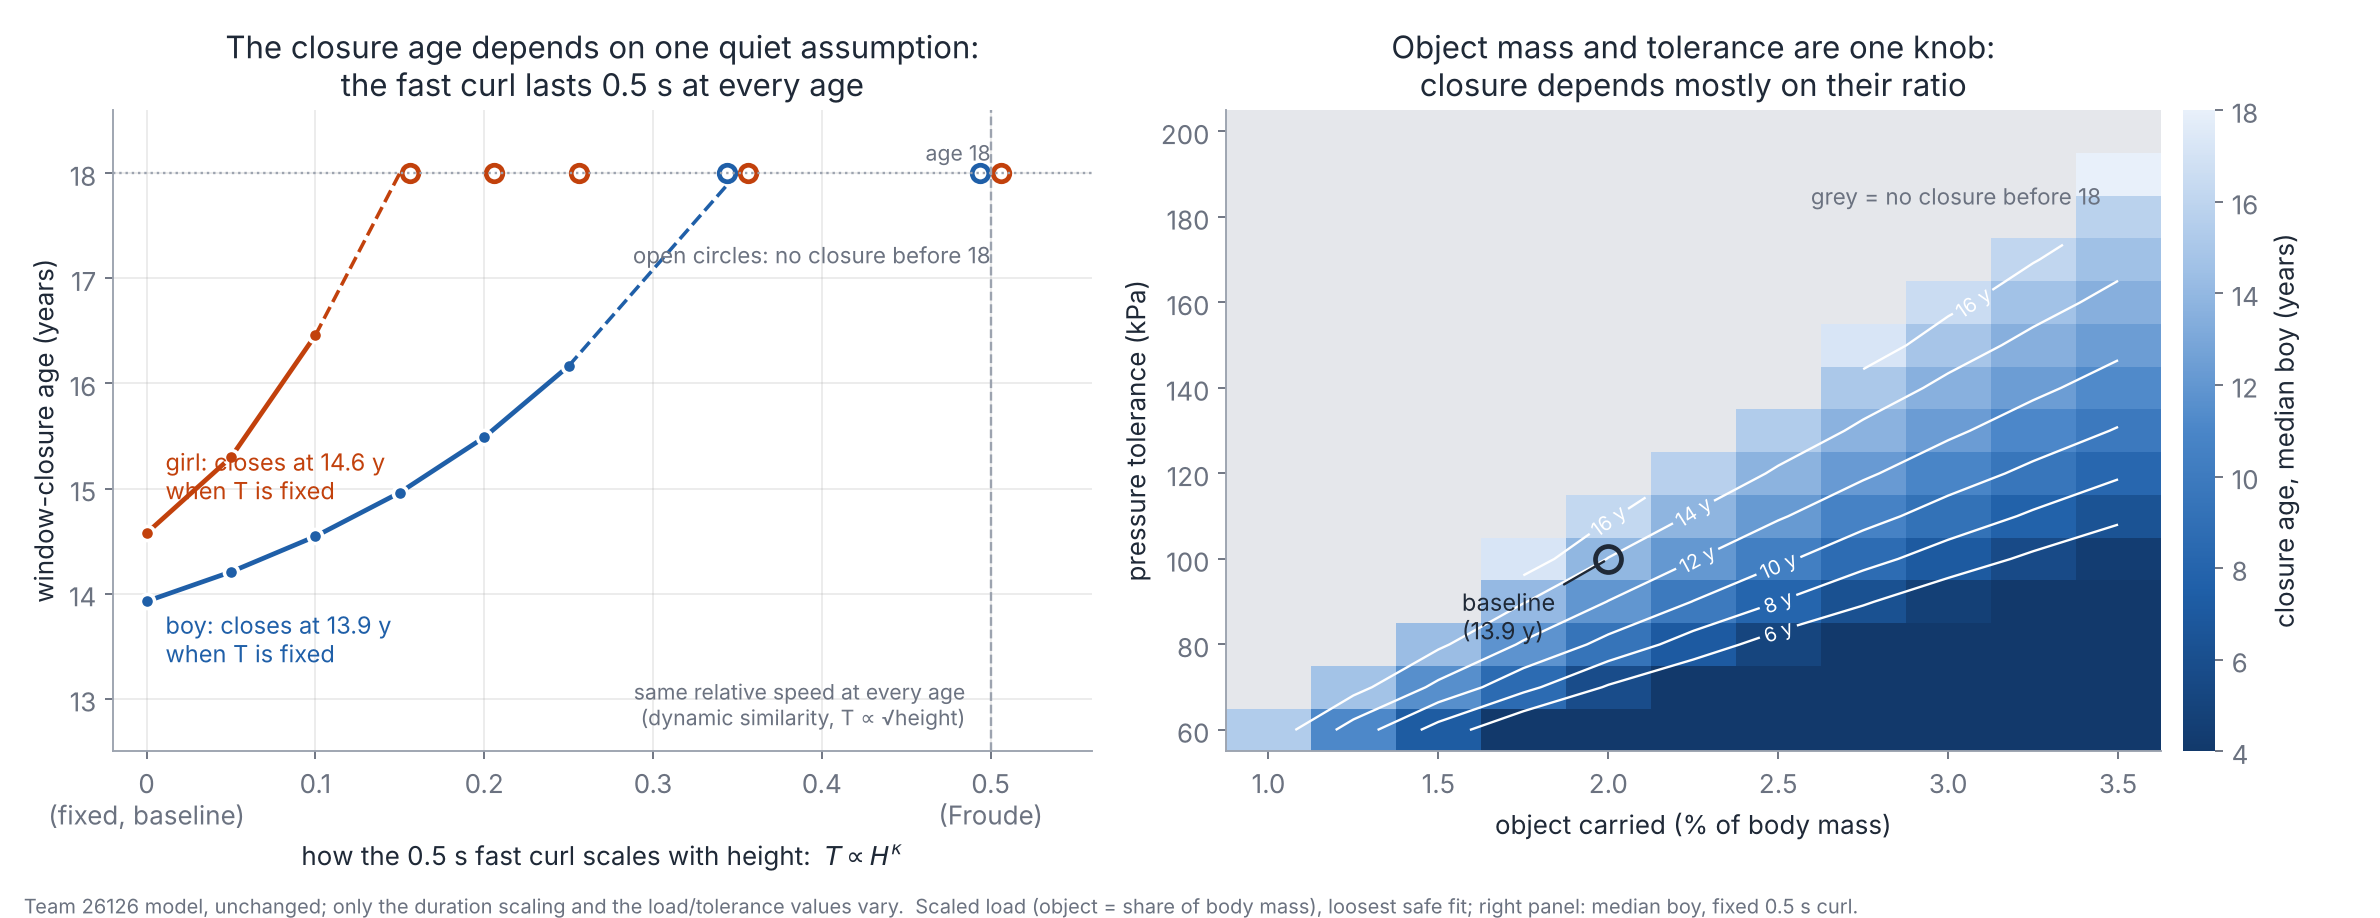
\includegraphics[width=\textwidth]{fig15_closure_hidden_assumptions}
\caption{Two assumptions behind the closure age. Left: closure age when movement time grows with height as $T\propto H^{\kappa}$. Right: closure age of a median boy over the object share and the pressure tolerance.}
\label{fig:hidden}
\end{figure}
\begin{figure}[t]\centering
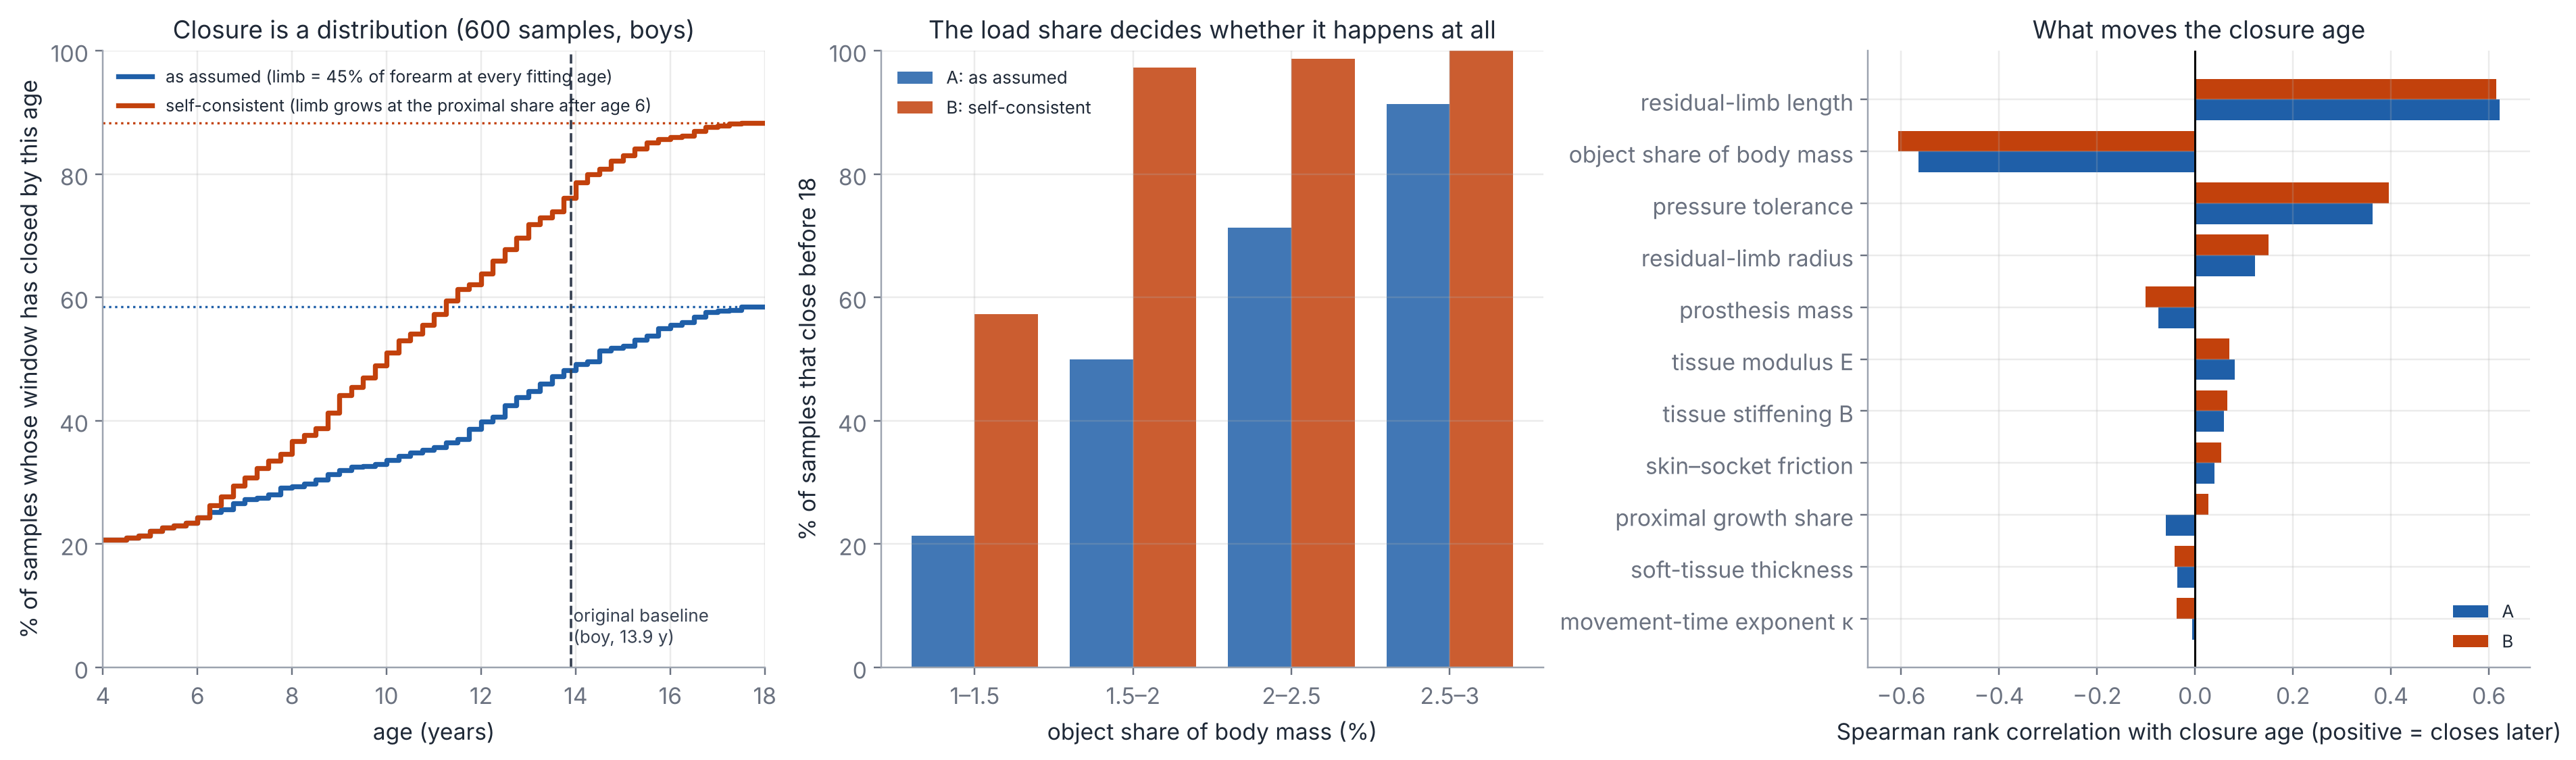
\includegraphics[width=\textwidth]{fig17_closure_probability}
\caption{Window closure as a distribution (boys, \cloMcN\ samples). Left: share of samples whose window has closed by each age, under the two readings of residual-limb growth; the dotted lines are the shares that close at all before 18. Centre: share that close before 18 by object share. Right: rank correlation of each input with the closure age.}
\label{fig:closureprob}
\end{figure}

\begin{figure}[t]\centering
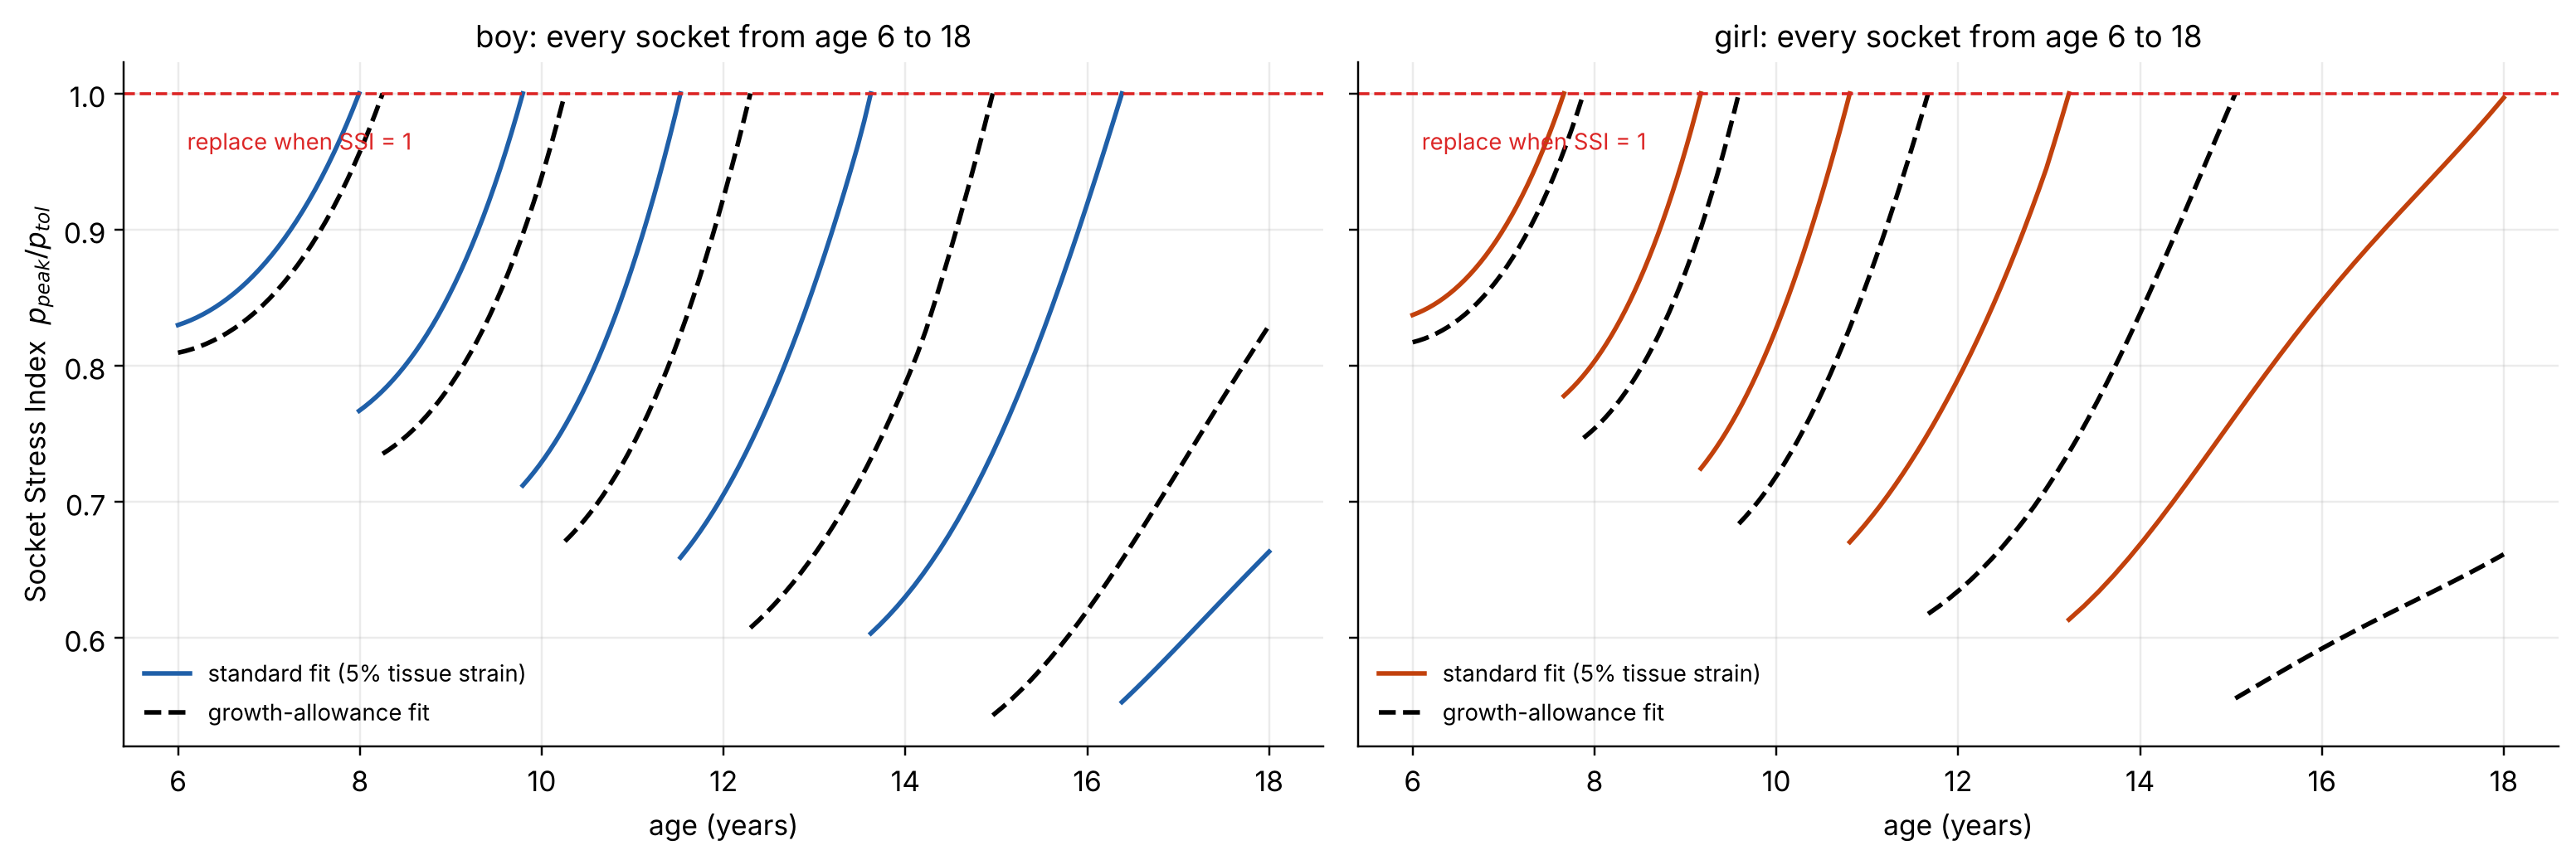
\includegraphics[width=\textwidth]{fig08_replacement_schedule}
\caption{Every socket from age 6 to 18 under standard and growth-allowance fitting.}
\label{fig:schedule}
\end{figure}
\begin{figure}[t]\centering
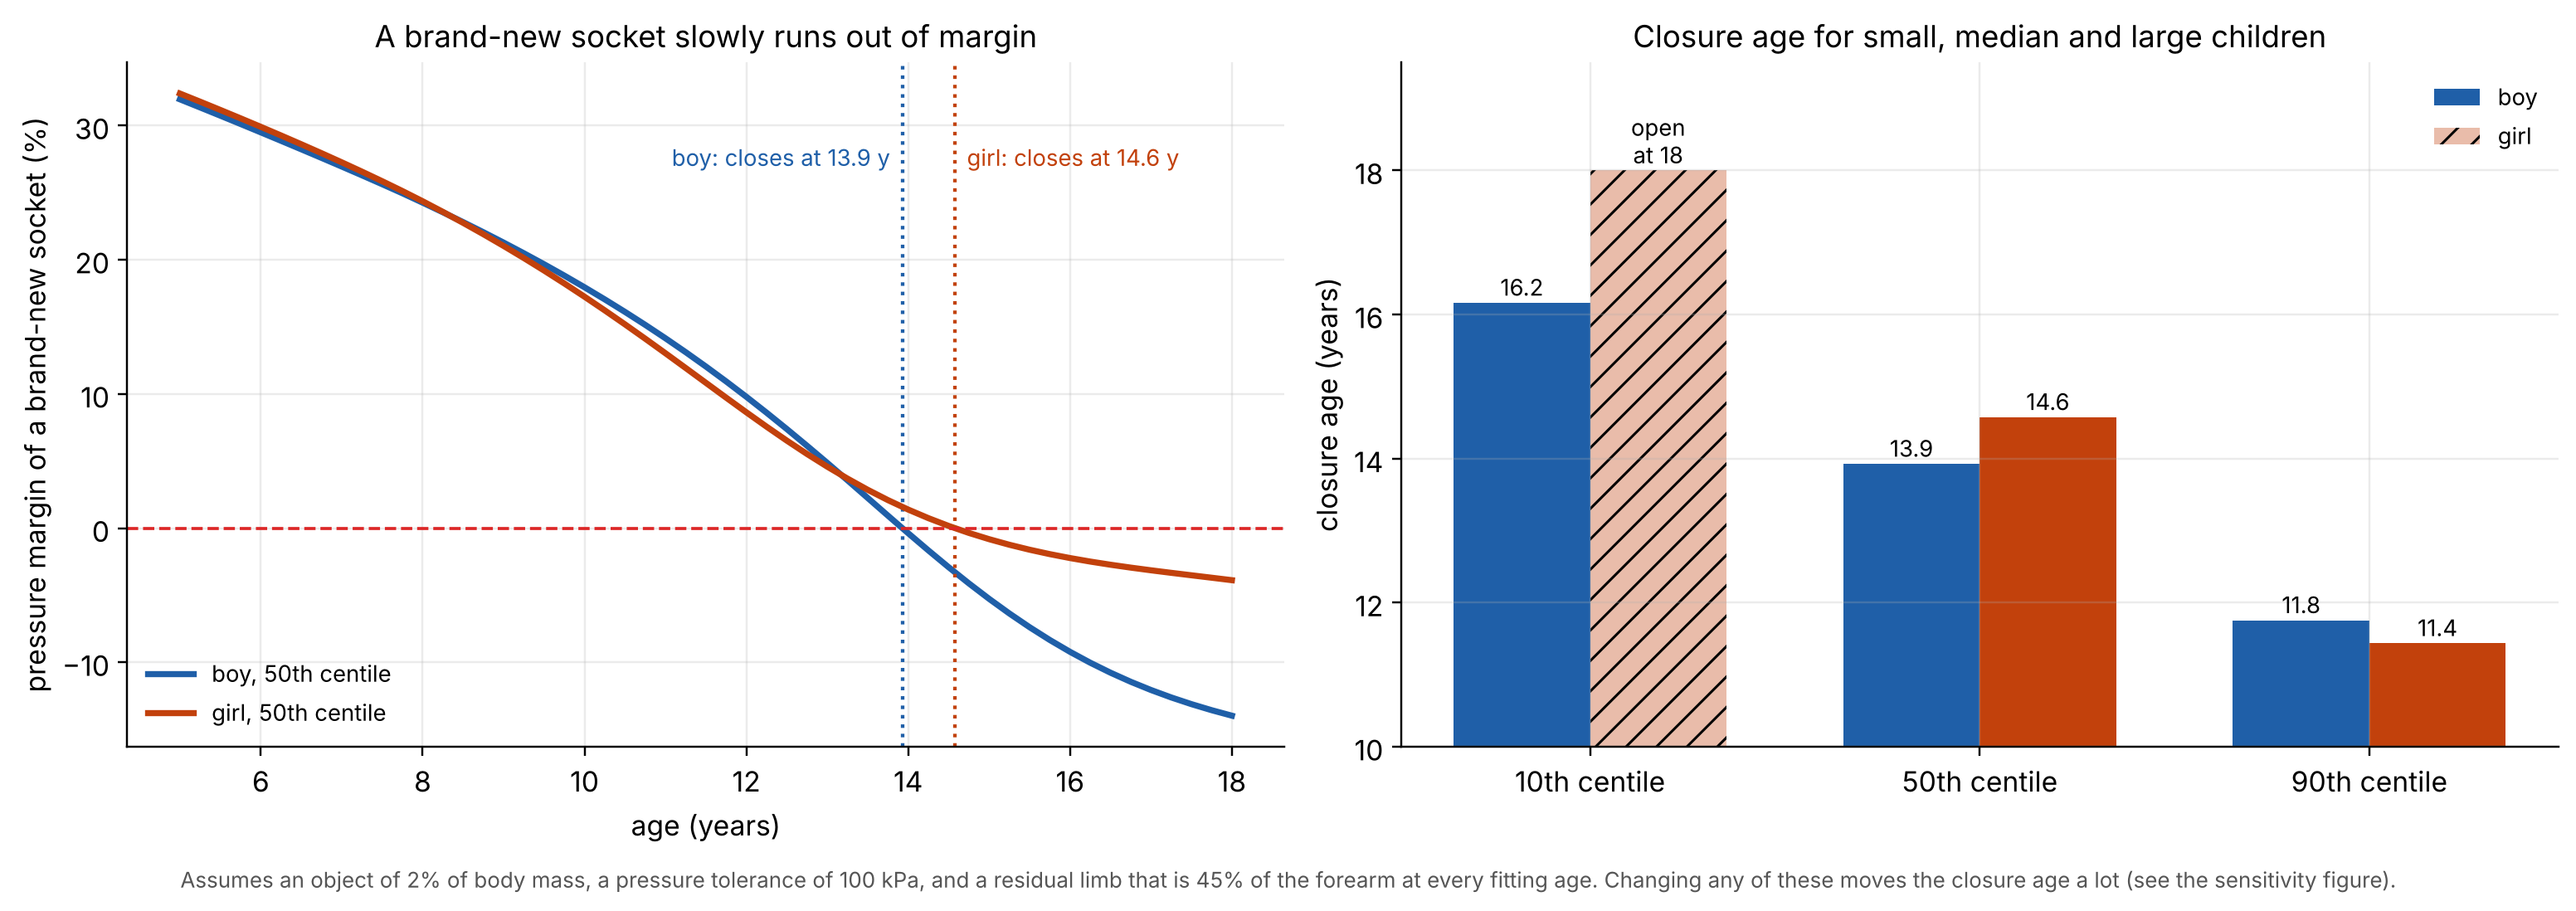
\includegraphics[width=\textwidth]{fig09_window_closure}
\caption{Left: pressure margin of a brand-new socket under growing loads. Right: closure age for 10th, 50th and 90th centile children.}
\label{fig:closure}
\end{figure}
\begin{figure}[t]\centering
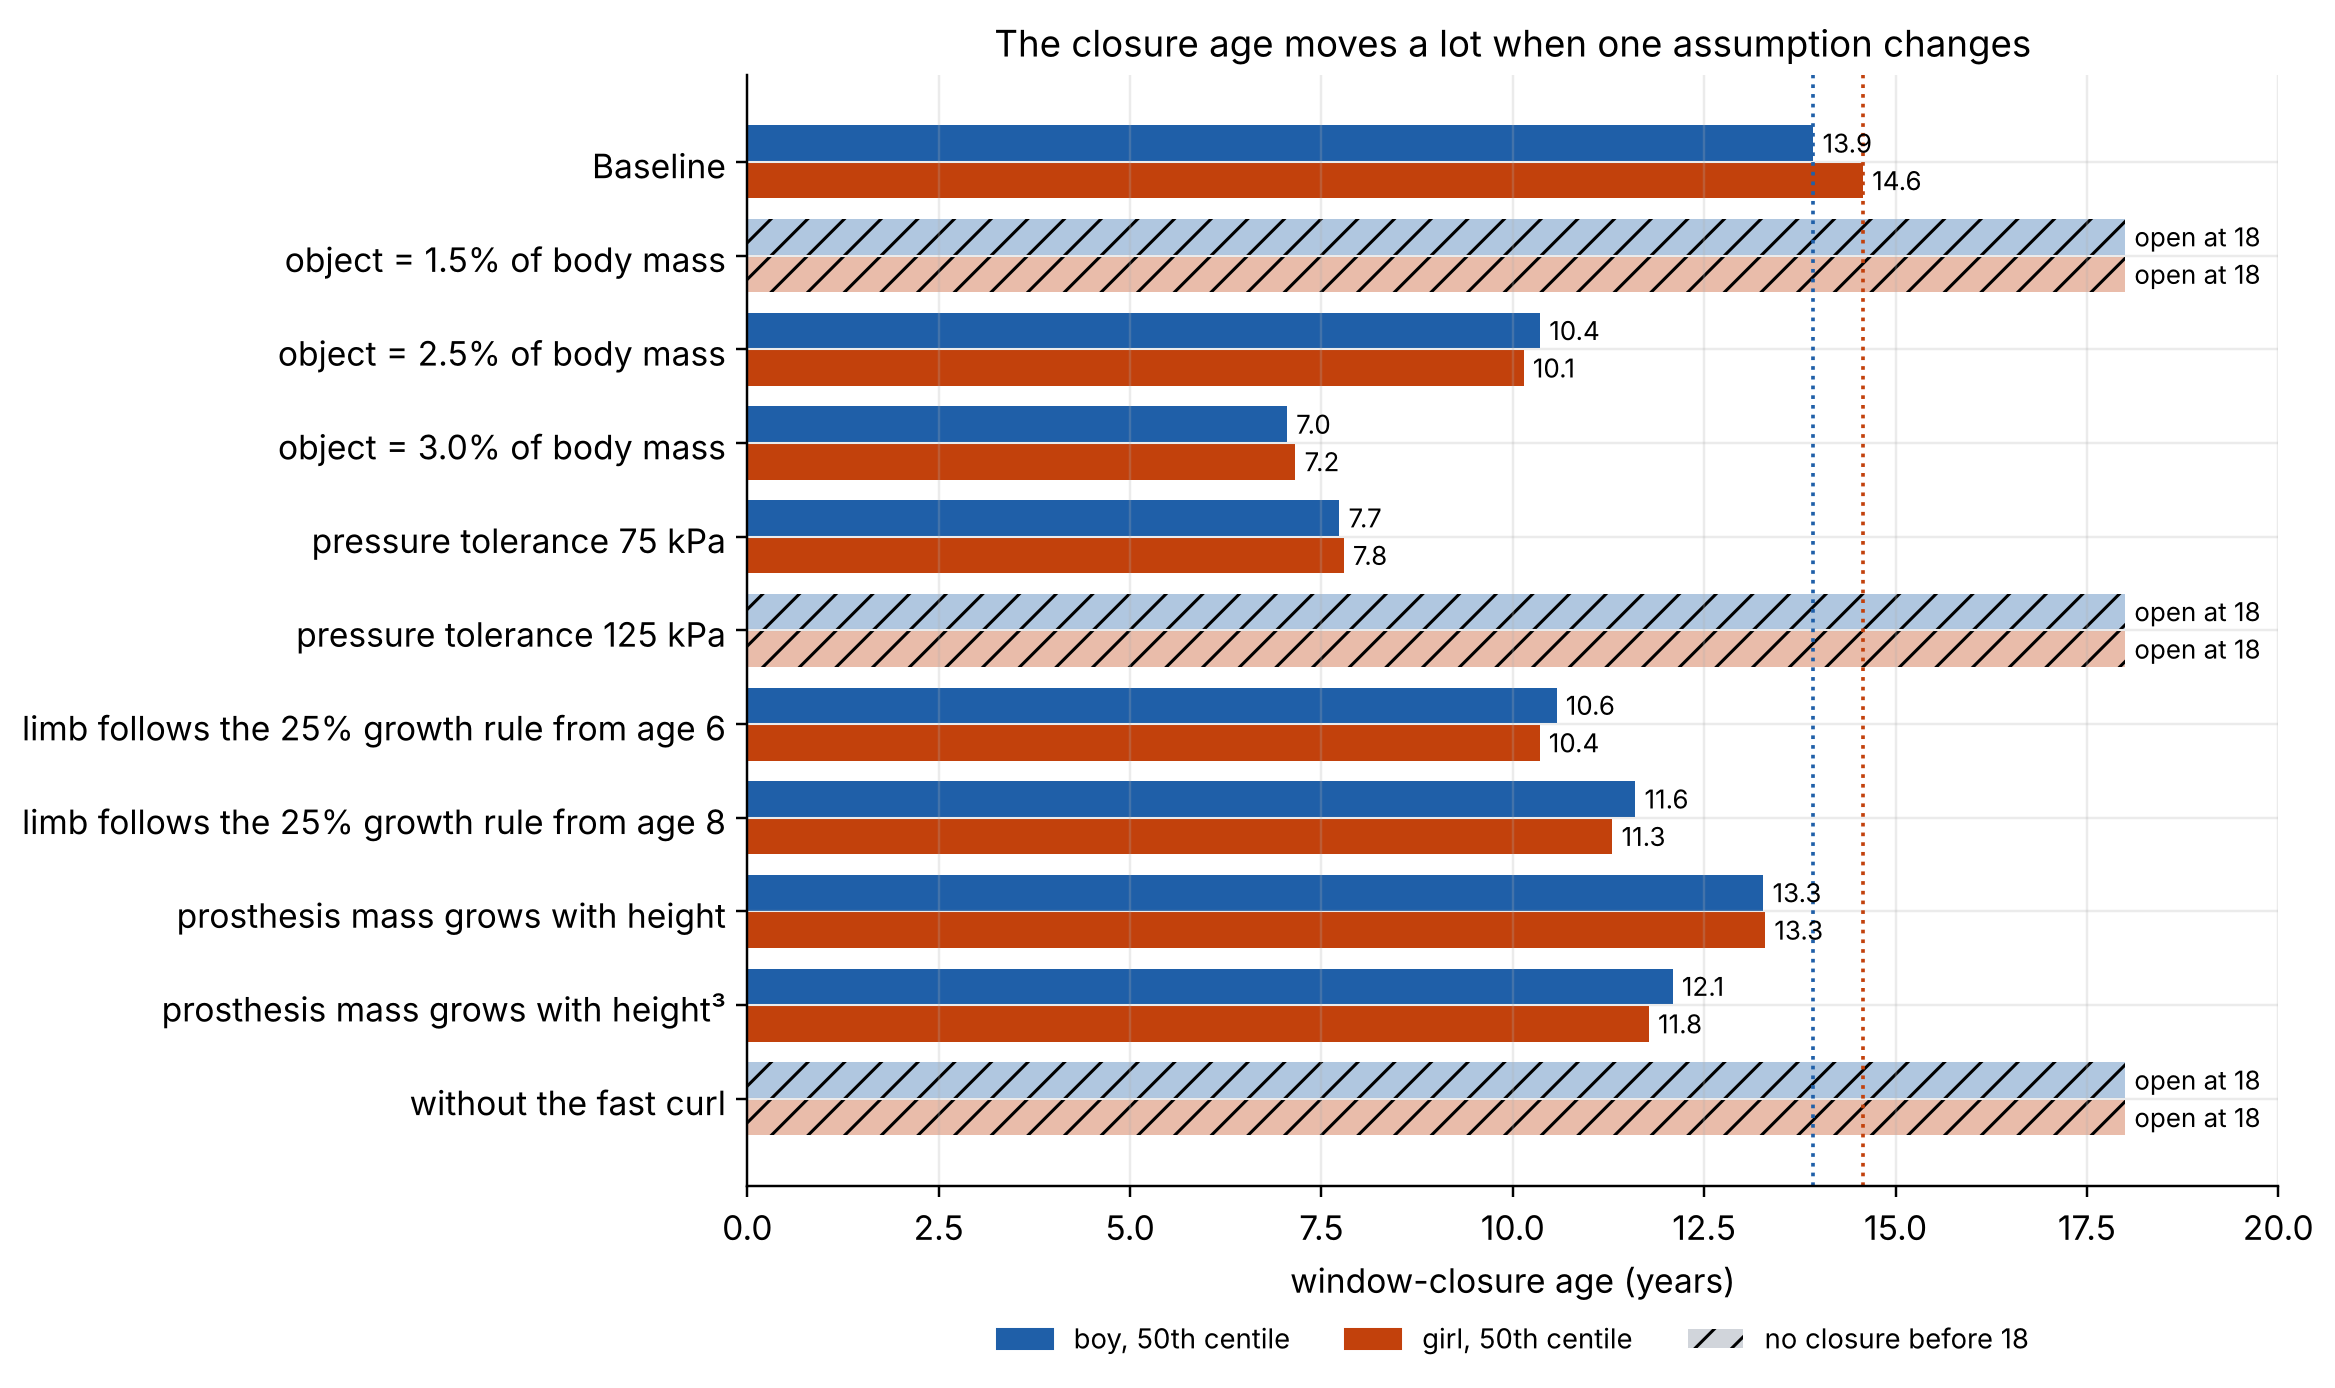
\includegraphics[width=0.85\textwidth]{fig14_closure_sensitivity}
\caption{Window-closure age for median children when one assumption is changed at a time. Hatched bars mean no closure before age 18. The dotted lines mark the baseline.}
\label{fig:firm}
\end{figure}

\section{Model 3: wider musculoskeletal effects}\label{sec:msk}
The prosthesis length is fixed at fitting while the intact forearm keeps growing. The resulting reach deficit $\delta=\ell^{\mathrm{intact}}_{\mathrm{grip}}-L_p$ must be compensated elsewhere. We model the simplest compensation, forward trunk lean $\beta=\arcsin(\delta/\ell_{\mathrm{trunk}})$, which adds a lumbar moment $0.678\,Mg\,(0.626\,\ell_{\mathrm{trunk}})\sin\beta$ \citep{winter2009}. Joint effort is torque divided by strength, with strength scaling as $M^{2/3}H$ (muscle cross-section times moment arm). If the socket fitted at 8 is not replaced, the deficit reaches \deficitEleven\,cm at 11 and \deficitTwelve\,cm at 12, requiring \leanEleven$^\circ$ and \leanTwelve$^\circ$ of trunk lean (Fig.~\ref{fig:msk}). Elbow effort (torque divided by strength) on the prosthetic side falls below that of the intact side as the child grows, because the prosthesis stays the same size while the child gets stronger. That could mean the prosthetic arm is being under-used, but it is an output of the model and not something we measured. The deficit at the scheduled replacement is only \deficitReplace\,cm, so timely socket replacement also protects the trunk. These are trends to watch rather than injury predictions: asymmetric loading and habitual lean are plausible contributors to posture and spine problems, but our model does not establish them.

\begin{figure}[t]\centering
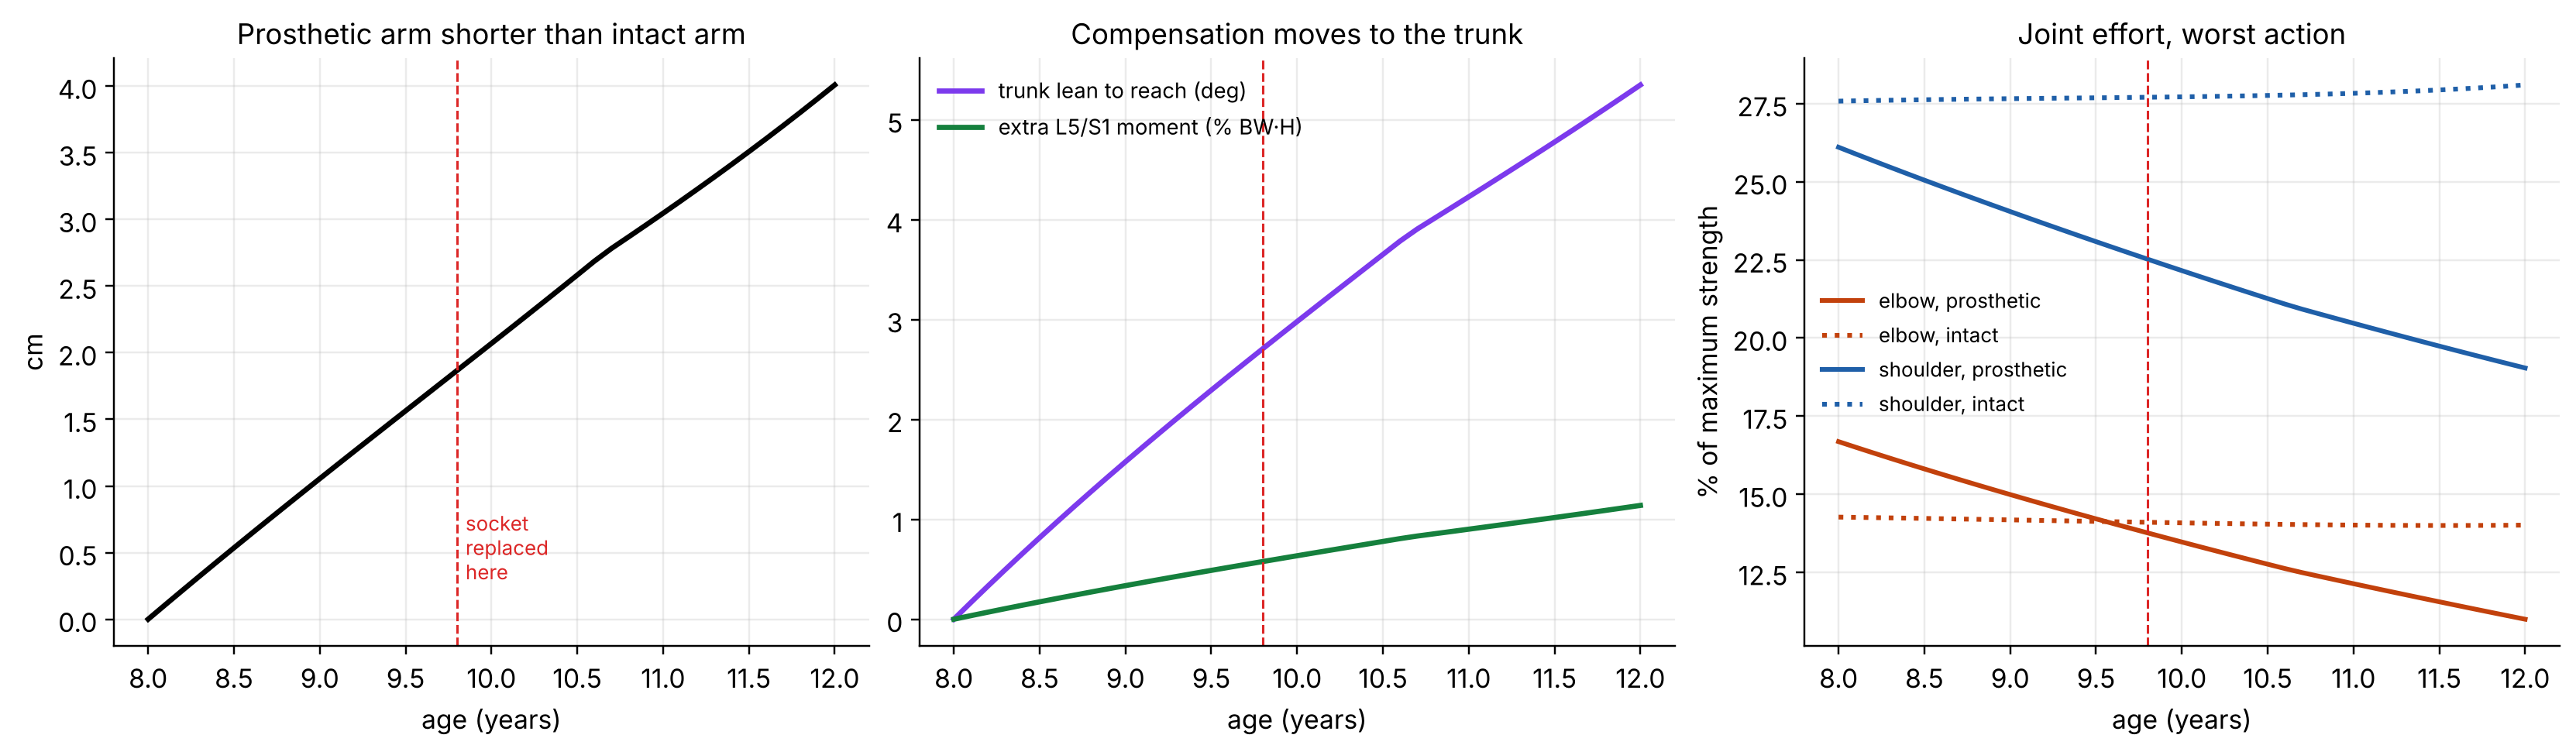
\includegraphics[width=\textwidth]{fig12_musculoskeletal}
\caption{Musculoskeletal consequences if the socket fitted at 8 is not replaced.}
\label{fig:msk}
\end{figure}

\section{Verification, sensitivity and uncertainty}\label{sec:verification}
\paragraph{Verification.} Nine of the ten checks in Table~\ref{tab:tests} are automated tests in the code repository (31 tests in all, run with \texttt{pytest}). The pistoning check is computed by \texttt{scripts/09\_verification.py} and is not a test.
\begin{table}[h]\centering\small
\begin{tabular}{@{}p{8.6cm}p{6.6cm}@{}}\toprule
Check & Result\\\midrule
Passive arm (no torque) conserves energy & drift $\energyDrift$ over 3\,s\\
Lagrange elbow torque $=$ Newton--Euler moment & max difference $\neError$\,N\,m\\
Torques fed back into the ODE reproduce the motion & max error \replayError$^\circ$\\
Line load satisfies force and moment balance & exact to $10^{-8}$\\
Static hold in Model~1 equals closed form of Model~0 & exact to $10^{-10}$\\
Growth ODE equals Preece--Baines closed form & $<10^{-6}$\,m\\
Growth-forced ODE system equals the algebraic interface model & relative difference $\odeStateErr$ over a socket life\\
ODE failure event equals scan-and-bisect lifetime & within \odeGap\ months in \odeN\ cases\\
Lifetime read from the pressure path equals the search & within \headroomGap\ months\\
Pistoning ODE $m\ddot u+c\dot u+ku=-A(t)$ is quasi-static & $f_n=\pistonFn$\,Hz $\gg$ 1\,Hz; slip \pistonSlip\,mm\\\bottomrule
\end{tabular}
\caption{Verification checks.}\label{tab:tests}
\end{table}

The pistoning check justifies treating the socket as quasi-static. The interface's natural frequency is about 40 times the frequency of lifting, so the dynamic slip equals the static value $-A/k$.

\paragraph{One-at-a-time sensitivity.} Varying each parameter by $\pm25\%$ (Fig.~\ref{fig:tornado}) shows that movement speed, residual-limb length and radius, and pressure tolerance dominate. Each of those four pushes a socket fitted at 8 to failure on the day of fitting when it is changed by 25\% in the wrong direction (a 25\% shorter residual limb, for example, consistent with the $L^{-2}$ law of Model~0). So our baseline sits fairly close to the tolerance for the fast curl.

\paragraph{Global uncertainty.} We sampled nine uncertain parameters over plausible ranges with \mcN\ Latin-hypercube samples \citep{mckay1979} (Fig.~\ref{fig:mc}). Patient-specific fitting raises the median lifetime from \mcStdMed\ to \mcIndMed\ months. In \mcDayOne\% of samples the fast curl already exceeds tolerance on the day of fitting. For those children the action itself, not growth, is the risk, and slowing it reduces $\Pi$. That is a large share, and it goes with the point above that the baseline sits near the tolerance. The stress index on the day of fitting, $S_0$, predicts lifetime well (Spearman $\rho=\mcRho$). This suggests a practical protocol: \emph{measure interface pressure during a brisk lift at fitting and use the model to schedule the next review}.

For the closure age the samples are much more spread out than the baseline suggests. \mcCloPinned\% were already closed at the youngest age we test (4 years) and \mcNever\% never closed before 18. The \mcCloBetweenN\ samples that closed in between did so at a median of \mcCloBetweenMed\ years (90\% range \mcCloBetweenLo--\mcCloBetweenHi). Counting the ``never'' samples as late, the median over all samples is \mcCloOverall\ years, close to our baseline, but \mcCloBeforeTwelve\% of samples close before 12 and \mcCloLate\% after 15 or never, and only \mcCloNear\% land within a year of the baseline. So closure happens before 18 in about two thirds of the samples, but the age at which it happens is poorly pinned down. Residual-limb length is the dominant driver (rank correlation \mcCloRho).

\begin{figure}[t]\centering
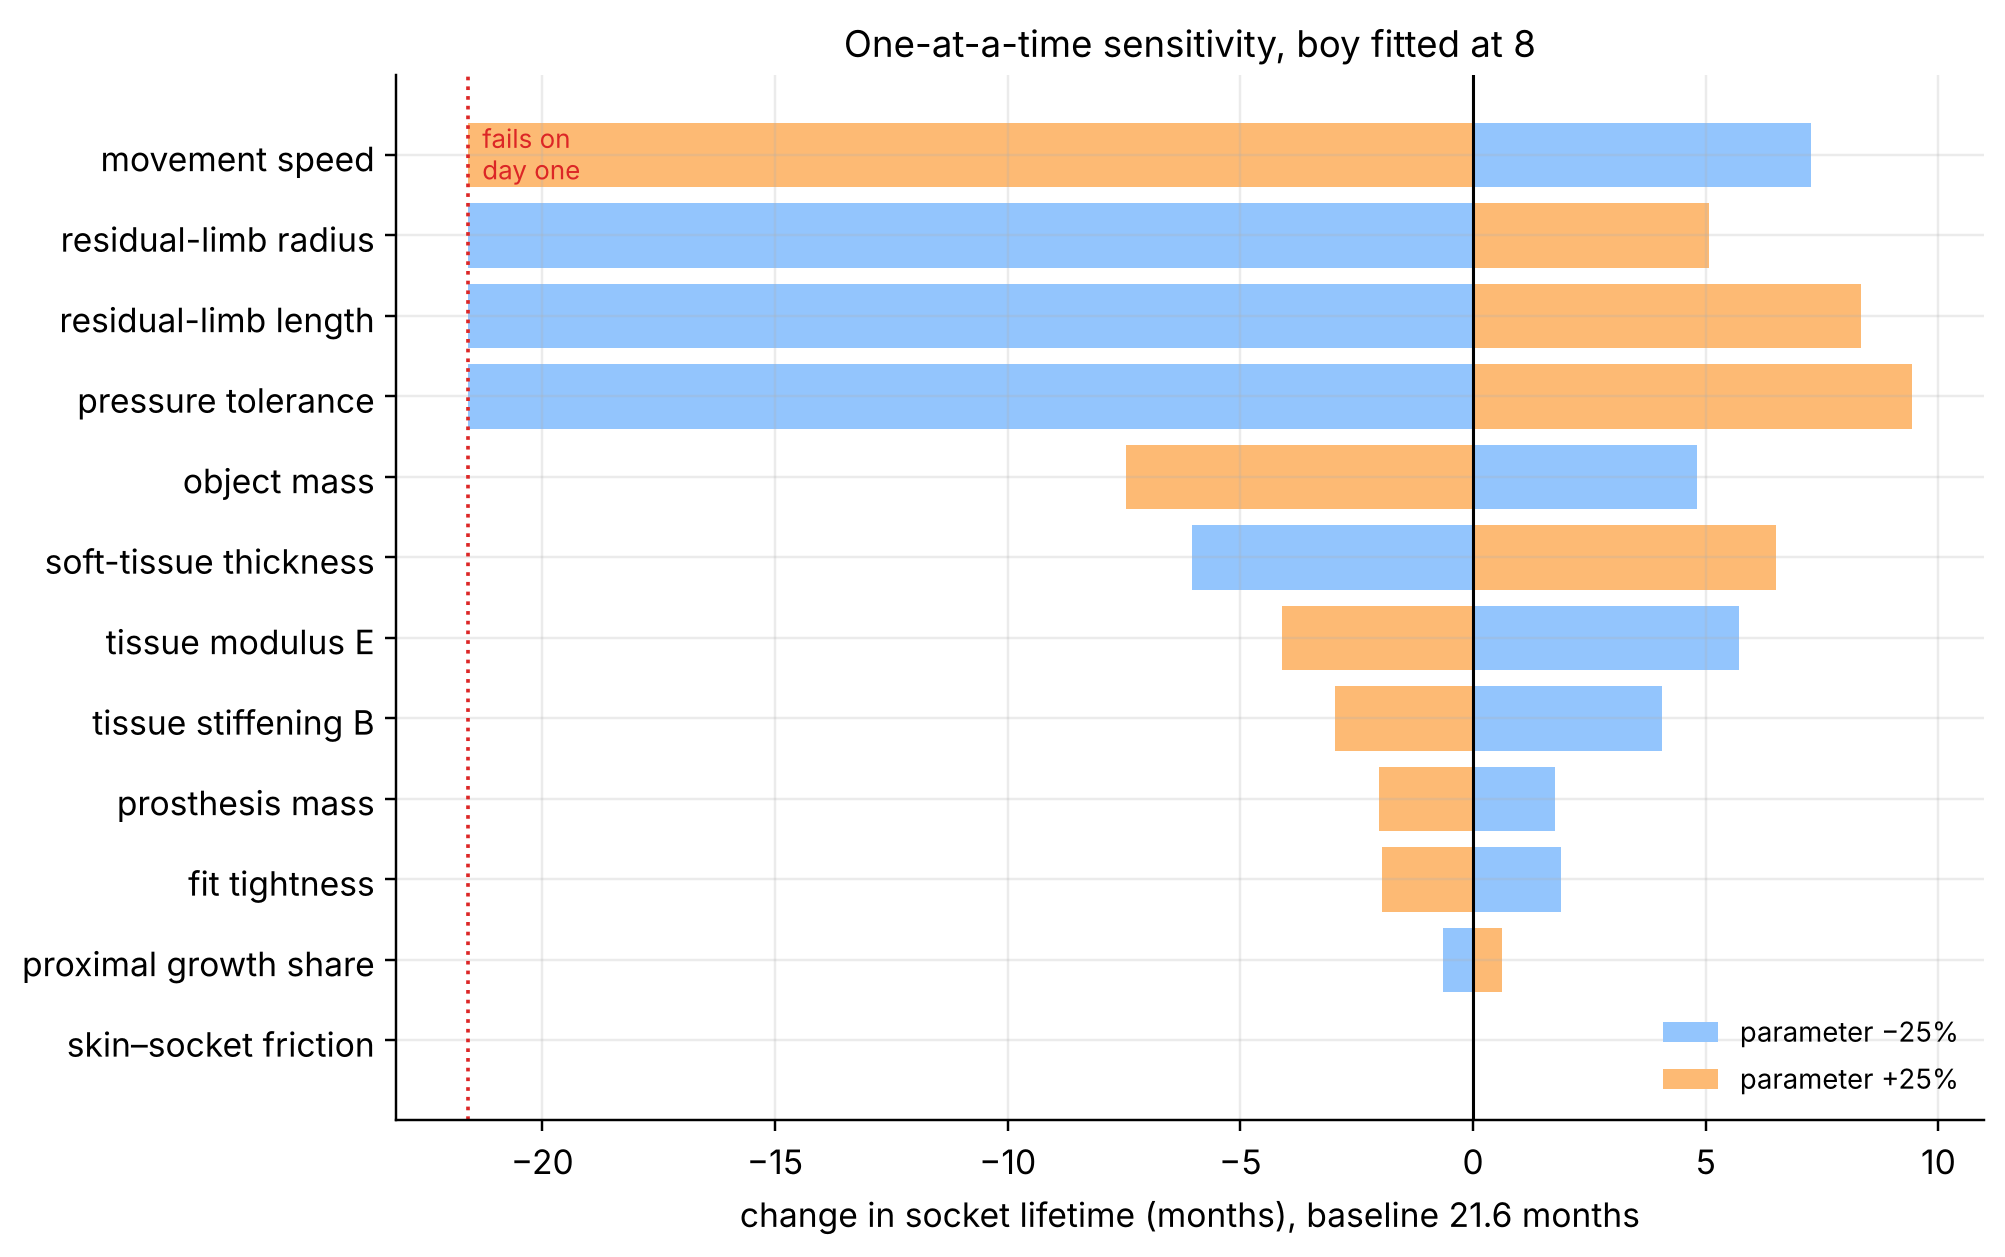
\includegraphics[width=0.62\textwidth]{fig10_tornado}
\caption{One-at-a-time sensitivity of socket lifetime.}
\label{fig:tornado}
\end{figure}
\begin{figure}[t]\centering
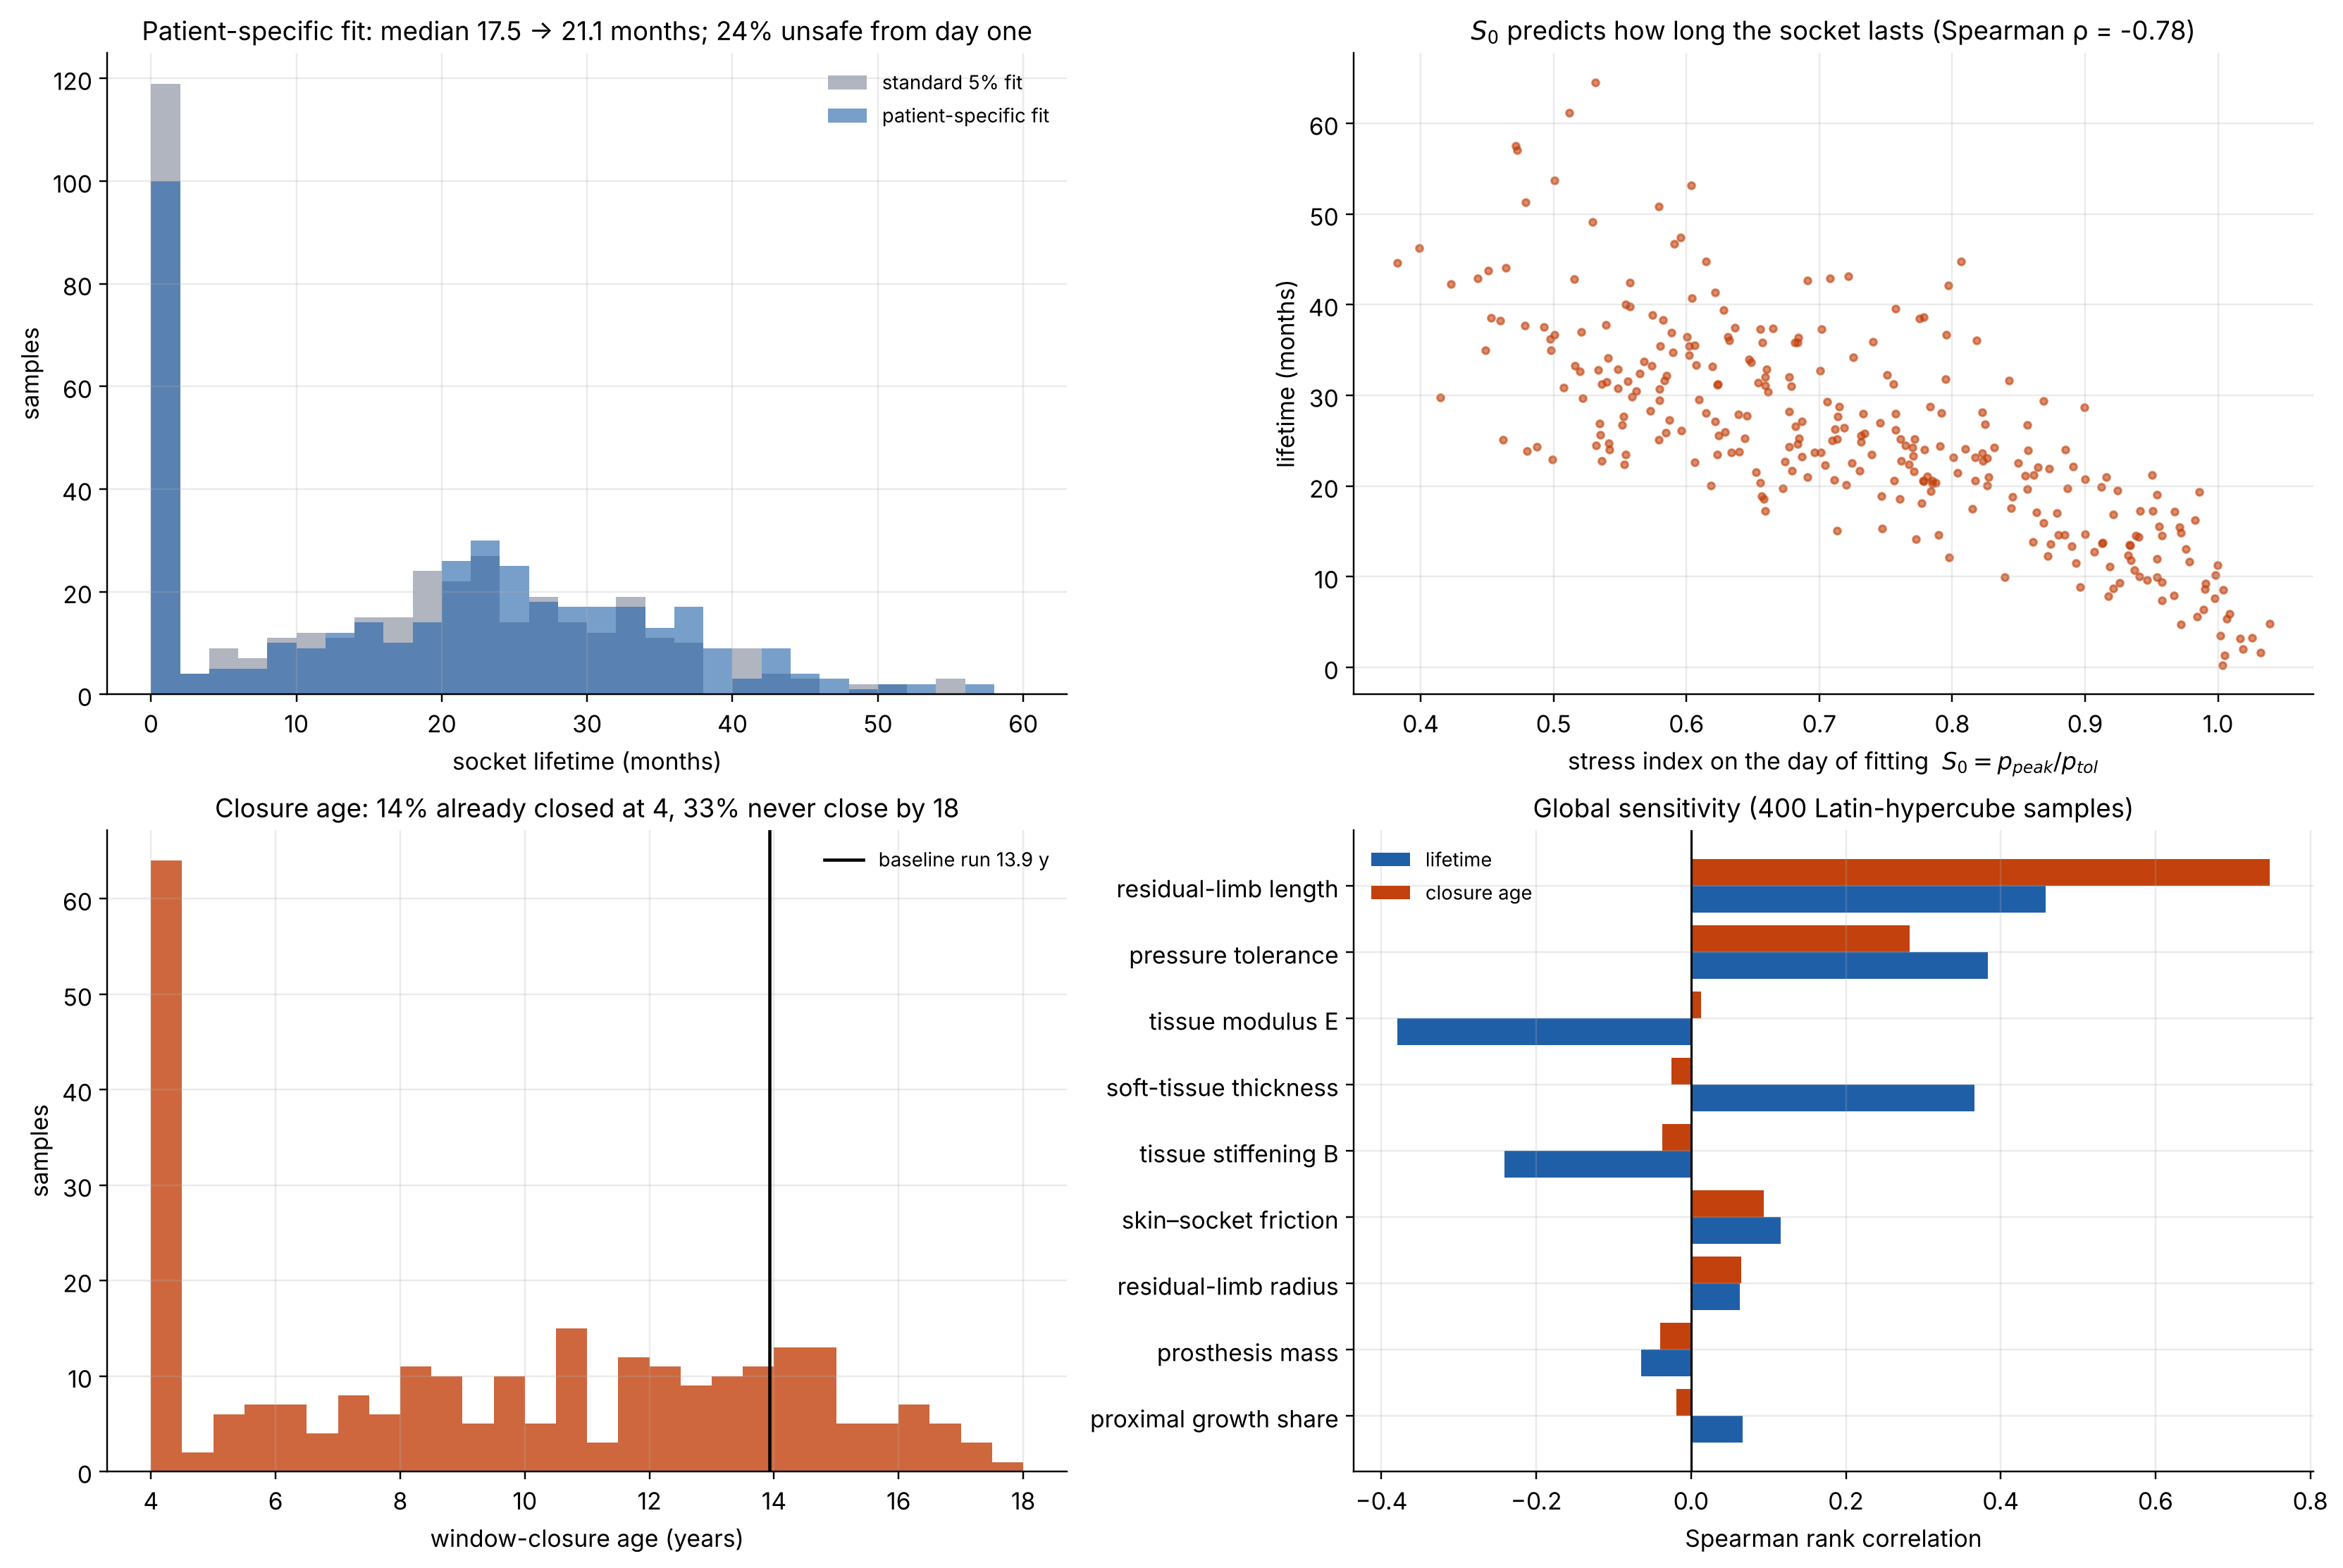
\includegraphics[width=\textwidth]{fig11_monte_carlo}
\caption{Global uncertainty and sensitivity from \mcN\ Latin-hypercube samples.}
\label{fig:mc}
\end{figure}

\section{Validation against published data}\label{sec:validation}
\paragraph{Scope.} Verification shows that we solved our equations correctly; validation asks whether they describe children. We looked for measured pressure histories of children's residual limbs and found none in the sources we could reach, so the pressure model itself cannot be validated against child data. What can be tested are the pieces around it (Table~\ref{tab:valid}, Fig.~\ref{fig:valid}). The comparison with replacement intervals is a consistency check of one tuned number, the tolerance, and not an independent test, and the clinical records are for lower-limb loss.

\begin{table}[t]\centering\small
\begin{tabular}{@{}p{3.0cm}p{3.5cm}p{4.4cm}p{4.0cm}@{}}\toprule
Quantity & Model & Published data & Reading\\\midrule
Replacement interval & \mcMedStd\ months (median, boy fitted at 8) & $16.4\pm9.9$ months, recommended 12--18 \citep{ghidini2025} & agrees; one tuned parameter; lower-limb data\\
Pressure tolerance & 100\,kPa (implied \impliedCyl--\impliedTap) & pain threshold \pptMean$\pm$\pptSd\,kPa, $n=50$, ages 4--12 \citep{nikolajsen2011} & \tolPct th percentile; plausible, not a test\\
Interface pressure & 37\,kPa static, 77\,kPa fast curl & about 40\,kPa, adult transhumeral \citep{razak2014} & same order of magnitude\\
Girth growth, 6$\to$17 y & +\girthBoyModel\% boys, +\girthGirlModel\% girls & arm +\girthBoyMuac\% / +\girthGirlMuac\%, wrist +\girthBoyWrist\% / +\girthGirlWrist\% \citep{ozturk2009,ozturk2017} & model a little high\\
Volume growth per year & \volSix--\volTwelve\% & up to 60\% \citep{ghidini2025poster} & growth alone is far below the extremes\\
Proximal growth share & 0.25 & 0.05--0.20 \citep{pritchett1991} & baseline slightly optimistic\\
Growth ODE (cm) & 0.28 in-sample & held-out \oosMin--\oosMax & descriptive, not predictive\\\bottomrule
\end{tabular}
\caption{What the model was compared with. Girth and volume data are cross-sectional or from lower-limb casefiles; see the text for each caveat.}\label{tab:valid}
\end{table}

\paragraph{Replacement interval.} Ghidini et al.\ analysed 62 casefiles from Cambodia and found growth-driven replacement every $16.4\pm9.9$ months and adjustment every $8.3\pm6.6$ months, against 12--18 and 3--6 months recommended in the literature \citep{ghidini2025}. The Monte Carlo median for a boy fitted at 8 is \mcMedStd\ months (Fig.~\ref{fig:valid}A). Among the samples that last beyond day one the mean is \mcLastMean\ months with a spread of \mcLastSd, similar to the observed SD, while \mcDayOneStd\% are over tolerance on the day of fitting. Only \mcWithinObs\% fall within one SD of the observed mean, because the model distribution has a spike at zero and a long upper tail. Equivalently, the tolerance that reproduces the observed mean is \impliedCyl\,kPa for a cylindrical socket and \impliedTap\,kPa for a tapered one, close to the 100\,kPa we fixed in advance. We stress that this calibrates one parameter with one number.

\paragraph{Is that tolerance reasonable?} In 50 children aged 4--12 the pressure-pain threshold, measured with a 1\,cm$^2$ probe, averaged \pptMean\,kPa (SD \pptSd) at the leg and was similar at the thenar, with no clear difference between younger and older children or between boys and girls \citep{nikolajsen2011}. Our 100\,kPa sits at the \tolPct th percentile of that distribution, the implied values at the \impPctCyl th--\impPctTap th, and the day-one peak of \pZeroEight\,kPa is \dayOnePPT\% of the mean threshold. A tolerance for repeated loading should lie below a single-trial threshold, so this is plausible, but a threshold at the leg and thenar is not a tolerance of a residual limb, and a protocol should use the clinician's own limit. In adult transhumeral sockets interface pressures of roughly 40\,kPa have been reported from F-Socket sensors \citep{razak2014}. Our child values (37\,kPa static, 77\,kPa for the fast curl) are of the same order, which says the magnitudes are plausible but does not test them.

\paragraph{Girth and volume growth.} Fit depends on how fast the limb thickens. Between ages 6 and 17 the model's radius grows by \girthBoyModel\% (boys) and \girthGirlModel\% (girls). The 50th-centile mid-upper-arm circumference in a Turkish school sample grows by \girthBoyMuac\% and \girthGirlMuac\% \citep{ozturk2009}, and wrist circumference by \girthBoyWrist\% and \girthGirlWrist\% \citep{ozturk2017}. The forearm lies between the two, so the model is probably a little high. Because the lifetime is $\ln R^*$ divided by the girth growth rate (Section~\ref{sec:ode}), girth growth 10--30\% slower than modelled would lengthen lifetimes by roughly 10--40\%; this follows from the formula and was not re-run. For volume, the model gives \volSix--\volTwelve\% per year at ages 6--12 from growth alone. That is far below the maximum of 60\% per year that the same group reported before replacement in below-knee casefiles \citep{ghidini2025poster}: real residual limbs change volume for reasons we do not model.

\paragraph{Growth-plate share.} Pritchett's radiographic study gives distal shares of about 80\% for the radius and 85\% for the ulna, rising to 90--95\% after age 8 \citep{pritchett1991}, so a residual limb keeps only 5--20\% of forearm growth. We used $\phi=0.25$. At $\phi=0.10$ and $0.20$ the lifetime of a socket fitted at 8 is \phiLifeLow\ and \phiLifeMid\ months instead of \lifeCyl, and the self-consistent closure age is \phiCloLow\ and \phiCloMid\ years instead of \sensLimbSixBoy\ (Fig.~\ref{fig:valid}D). The baseline is therefore slightly optimistic about longitudinal growth, which in this model helps the socket.

\paragraph{Growth curve.} The Preece--Baines ODE reproduces the CDC median to \pbRmseBoy\,cm RMS, but that is in-sample. Fitted only to data from before the growth spurt it does not predict the spurt: held-out RMS errors are \oosMin--\oosMax\,cm. We therefore use it as a smooth, differentiable description of the reference curve and not as a predictor for an individual child.

\paragraph{What would settle it.} A study that records interface pressure during a brisk lift at each fitting and again at the next clinic visit would give $P(0)$, $T(x)$ and the tolerance directly. Until then, what this paper offers is the shape of $P(t)$, the girth budget, and the dependence of closure on the load share, rather than a calibrated age.

\begin{figure}[t]\centering
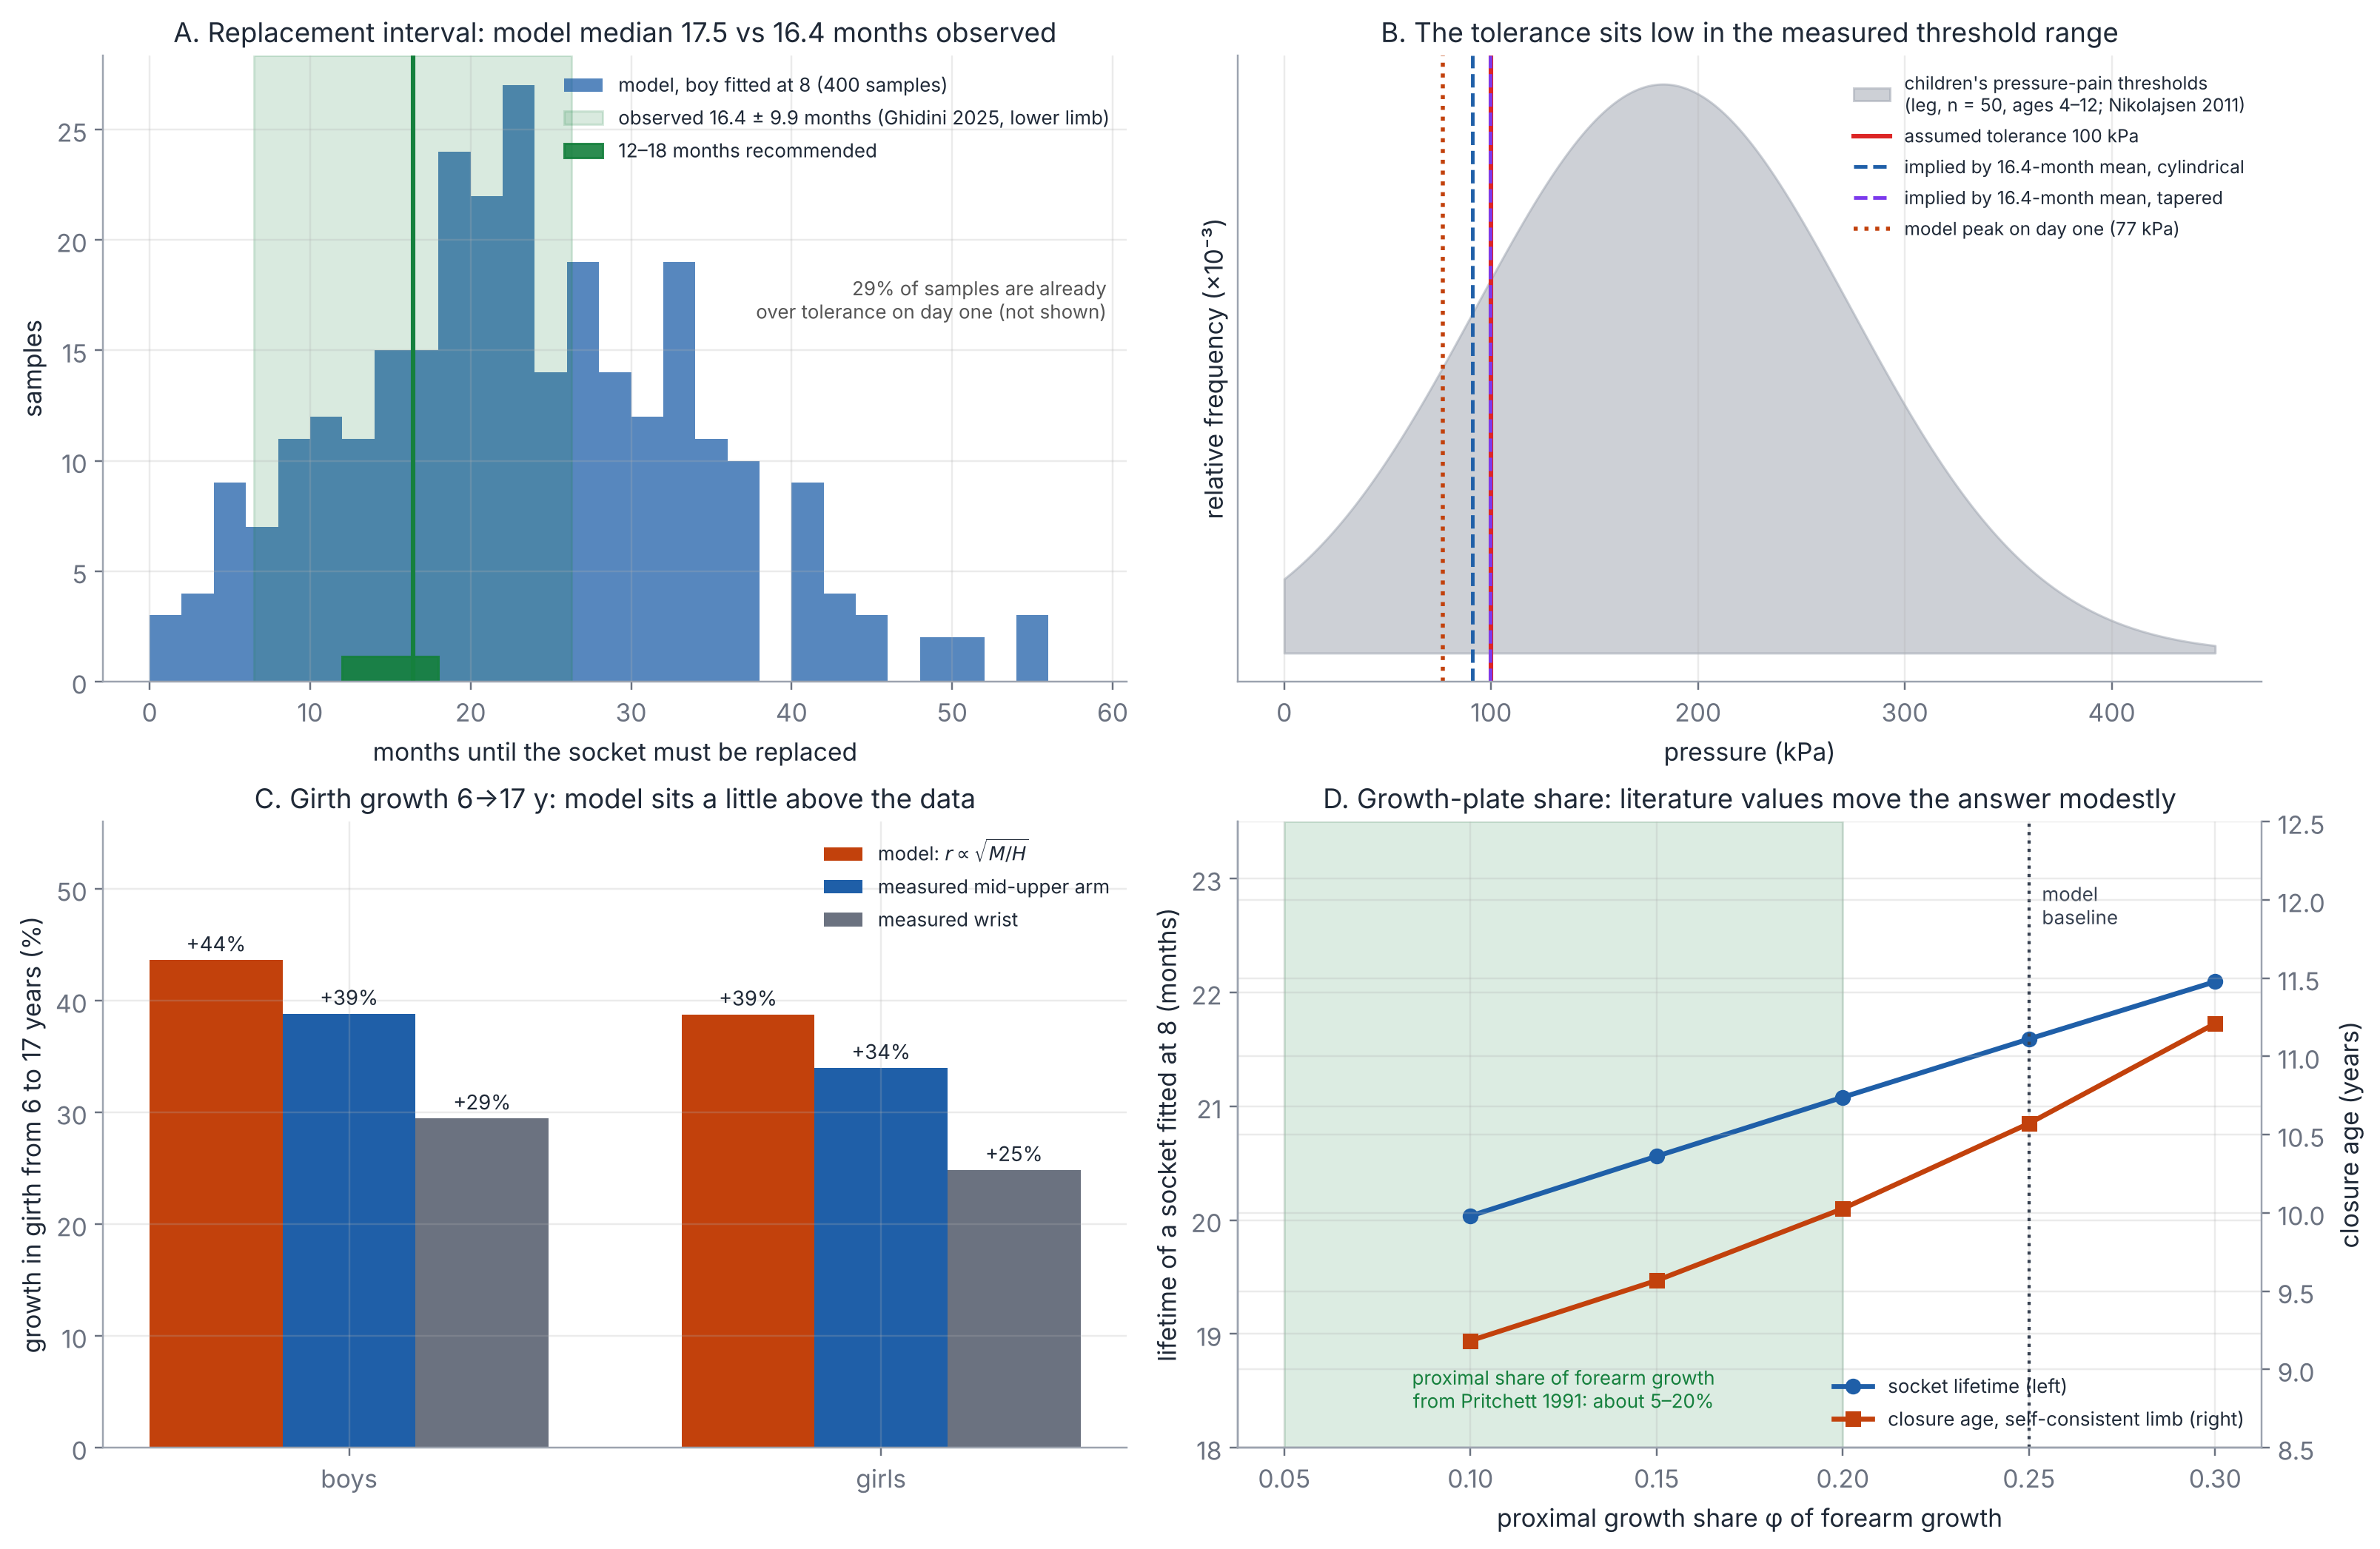
\includegraphics[width=\textwidth]{fig19_validation}
\caption{Comparison with published data. A: replacement interval, model samples against Ghidini et al. B: assumed and implied tolerance against children's pressure-pain thresholds. C: girth growth. D: effect of the proximal growth share.}
\label{fig:valid}
\end{figure}

\section{Discussion}
\paragraph{Answers to the problem.}
(1)~For a set of simple planar lifts, the interface load is set by a moment over the square of the engaged length, and fast motion amplifies it linearly in $\Pi$.
(2)~Growth changes the interface through girth (tissue compression or ride-up) far more than through length, because the residual limb has lost its distal growth plates.
(3)~There are two points of change. Routine replacement follows a tolerance-free pressure path: for a boy fitted at 8 the peak pressure is 25\% higher after \tPlusBoyCyl\ months in a cylindrical socket and \tPlusBoyTap\ in a tapered one, and across ages and sexes after \tPlusMin--\tPlusMax\ months, which brackets the 12--18 months used in practice. With our assumed tolerance this is \lifeTap--\lifeCyl\ months for a boy fitted at 8 (13.5 to 37 months across ages, sexes and socket types). A substantial change, the closure of the fit window, is a conditional event: it needs an everyday load that grows with the child faster than movement slows, it occurs before 18 in \cloAclosed--\cloBclosed\% of our samples with a median age of \cloBmed--\cloAmed\ years, and it needs a redesign rather than a refit.
(4)~Beyond the socket, an outgrown prosthesis shifts work to the trunk in our model, and it may leave the elbow on the prosthetic side under-used. These are trends to watch, not predictions of injury.

\paragraph{What we trust.} Each layer is built on the previous one and checked against it, and the growth input is real reference data. Within the model, the scaling laws and the girth budget follow from geometry and the tissue law, and the numerical results confirm them. The dependence on $\Pi$ is useful above $\Pi\approx0.3$, with the caveat given in Section~\ref{sec:dynamics}. The time scale of replacement and the order of magnitude of interface pressure agree with published records (Section~\ref{sec:validation}). The tolerance, the object share and the way movement time scales with size have no child data behind them, so we state results in a form that stays valid when they are replaced. We also tried to break our own headline result, and that is why this report says how far it can be trusted.

\paragraph{Weaknesses and future work.} The biggest weakness is that the tissue parameters, the pressure tolerance and the load (2\% of body mass) are working assumptions in a plausible range, not measurements on children, and the closure age depends strongly on them (Fig.~\ref{fig:firm}). They should be calibrated with pressure-sensor data from real fittings; we found no such measurements for children's residual limbs. The clinical replacement data we compare with are for lower-limb loss, and our girth growth is a little higher than measured arm and wrist growth while real volume changes are far larger than growth alone. Our baseline also sits close to the tolerance for the fast curl, so in about a quarter of the Monte Carlo samples it fails on the day of fitting. Height and weight share one centile, so a ``90th-centile child'' is both tall and heavy. Adult segment ratios understate young children's relative head and trunk size. The baseline treats the residual limb as a fixed share of the forearm at every fitting age, which does not match the growth rule used after fitting; we therefore report closure under both readings (Fig.~\ref{fig:closureprob}). The Preece--Baines ODE describes the reference curve but does not predict it out of sample. The socket is idealised as cylindrical or uniformly tapered, and we look at only four planar actions, so a finite-element socket, daily volume fluctuation and three-dimensional motion are natural next steps. Bone overgrowth of the residual limb, a known complication after acquired amputation in children, could be added as a slow length change.

\section*{Use of AI tools}
As the COMAP policy requires, we report that AI assistance was used throughout this project. Claude (Anthropic) helped us to design the model, write and run the code, and draft and edit this report, our video script and our slides in November 2026. In a final editing pass it also reviewed the work, rewrote wording that sounded machine-written, added the closure-sensitivity analysis (Fig.~\ref{fig:firm}) and corrected several overstatements in an earlier draft of this report. In a second pass it added the tolerance-free pressure path (Fig.~\ref{fig:headroom}), the growth--load system as ODEs with failure events (Section~\ref{sec:ode}), the closure probability study (Fig.~\ref{fig:closureprob}) and the comparison with published data (Section~\ref{sec:validation}), and extended the automated tests from 19 to 31. The tools, versions, prompts and outputs are listed in our separate Report on Use of AI Tools. All equations, code and results were checked by the team, and the code includes automated tests of the main mechanical results.

\bibliographystyle{plainnat}
\bibliography{references}
\end{document}
